\chapter[The advection effect]{The advection effect as a driver of microbial biogeography}
\label{ch:advection}

\previouslypublished{Sections of this chapter have been previously published in}

\section{Abstract}

The distribution and abundance of marine microbes are shaped by environmental factors and spatial separation.
The physical transport of cells by ocean currents (advection) is also frequently invoked when describing marine microbial biogeography, but the role of advection has never been directly confirmed or measured.
This chapter describes a study in which the microbial communities at 25 sites in the Southern Ocean were sampled and compared to a model of particle advection between the sites, as well as their spatial and environmental distances, in order to test for the existence of an ``advection effect''.
An advection effect was confirmed, and found to explain at least 7\% of variation in community composition.
Further investigation confirmed that this effect was directional, and likely represented an increase in the colonisation of distant sites by small numbers of cells.
This study contributes a novel and replicable method for examining the effect of advection on marine microbes.
By demonstrating the existence of an advection effect, it also provides further evidence that microbial dispersal potential is far from total, and supports the role of ocean currents in shaping marine microbial ecosystems.

\section{Introduction}

\subsection{Distance and environment effects in microbial biogeography}

The central goal of microbial biogeography is to understand how the distribution and abundance of microorganisms are shaped by their physical context.
The Baas Becking hypothesis --- that ``\textit{everything is everywhere}, but, \textit{the environment selects} \cite{Becking:1934um, deWit:2006de}'' --- posits that the rapid dispersal of microorganisms means microbial community structure is determined entirely by environmental selection.
The assumption that microorganisms are effectively free from barriers to dispersal (``everything is everywhere''), while not universally agreed upon, has been maintained into the 21st century \citep[e.g.][]{Finlay:2002er}.
This stands in contrast to macroorganism biogeography, which has long been recognised as being under the control of historical (in addition to contemporary environmental) factors, particularly spatial influences such as barriers to dispersal.

In recent years, however, studies of microbial biogeography have begun to show that historical factors may also shape the distribution of microorganisms \cite{Martiny:2006jy}. 
One of the first and best known reports of microbes exhibiting a non-random spatial distribution was the finding by \citet{Cho:2000tn} that the genetic distance between fluorescent \genus{Pseudomonas} strains in soils was correlated to the spatial distance (a ``distance effect'').
(This study, among others \cite{Ramette:2007bb,Storch:2008tq}, also demonstrated the importance of taxonomic resolution in describing such biogeographic patterns.)
Further examples were soon discovered; \citet{Martiny:2006jy} found 23 studies published between 2000--2006 that described microbial distance effects, on spatial ranges from 2 m to 20,000 km.
Moreover, in some cases a distance effect could be identified even when contemporary environmental selection (an ``environment effect'') did not have a statistically significant effect on community composition.

When combined with the environment effect, distance effects explain some but not all variation between microbial communities, and the mechanism(s) by which a distance effect arises are not always clear \cite{Hanson:2012cb}.
Allopatric speciation (i.e.\ the divergent evolution of geographically isolated populations) is a likely cause in at least some cases.
\citet{Whitaker:2003dz} elegantly demonstrated this in a study on the hyperthermophilic archaeon \genus{Sulfolobus}, finding that isolates from geothermal springs across the Northern Hemisphere exhibited genomic differentiation strongly correlated to geographic distance.
Their results suggest that \genus{Sulfolobus}' highly specialised hyperthermophilic and acidophilic adaptations mean that the geographic distance between hot springs is a strong barrier to dispersal.

Other potential factors leading to incomplete dispersal of microorganisms include differences in population density and dispersal potential.
A common argument for the universal dispersal of microbes is that their large population sizes and fast growth rates mean that individually unlikely dispersal events become more probable when large populations are considered \cite{Finlay:2002er}.
However, the underlying assumption --- that all microbial species have large population densities and rapid growth --- is undermined by the ``rare biosphere'' of low-abundance microbial taxa \cite{Sogin:2006er}.
Moreover, different microbial species may have different dispersal potentials due to their biological properties.
For example, bacteria able to sporulate or that are otherwise resistant to long periods of environmental stress were found to exhibit a stronger distance effect in Australian soils \cite{Bissett:2010wj}.
Cell size may also play a role \cite{Martiny:2006jy}.

\subsection{Water mass endemicity and advection of marine microorganisms}

In the ocean, several recent studies have found that microbial communities can be endemic to hydrographically distinct water masses.
Surveys in the Arctic \cite{Galand:2009hy} and North Atlantic \cite{Agogue:2011fm} oceans have found that bacterial assemblages within the same water mass can be similar across a range of thousands of kilometres, but assemblages can differ between water masses across a range of hundreds of meters.
Water masses are defined by their distinct physicochemical properties, so such patterns do not directly imply the existence of factors beyond environmental selection.
However, in some cases a water mass-community relationship has been shown to persist even when environment effects are statistically controlled for \cite{Hamilton:2008tp, Hamdan:2013ko}.

During the study on the biogeographic effect of the \ac{PF} described in \secreft{ch:polarfront}, it was found that microbial communities in surface waters of the Mertz Glacier region, a site of deep water formation, were very similar to those at the bottom of the water column, despite the very different environmental conditions (see \secreft{ch:deepwaterformation}).
One hypothesis explaining both this observation and water mass endemicity is that microbial assemblages are influenced by the advection (physical transport) of cells by ocean currents. 
Higher dispersal rates cause the microbial community composition at a given site to increasingly resemble the dispersed colonisers, and less reflect local environmental selection and stochastic effects such as genetic drift \cite{Hanson:2012cb}.
Hence, it would be expected that locations that are closely connected by advection (e.g.\ those within the same water mass, or different levels of the water column at a site of deep water formation) would have more similar compositions than those that are not, even when the environment effect is accounted for.
Indeed, advection is often invoked to explain observations of microbial diversity or abundance which do not seem attributable to environmental selection \citep[e.g.][]{Sul:2013in, Ghiglione:2012ei, Giebel:2009hr, Lauro:2007bf}.
The exchange of very small volumes of water between marine microbial mesocosms has been found to greatly reduce their \textbeta-diversity even under consistent environmental conditions \cite{Declerck:2013cz}.
This suggests that advection of even small numbers of cells could have a large homogenising effect independent of environmental selection.
However, the existence of a relationship between advection and community composition that obtains independent of environment and distance effects has not been directly tested.

\subsection{Aims and approach of this study}

The \ac{SO} is composed of several water masses, which are physicochemically distinct but linked by circulation (see \secreft{ch:intro} for a full description; see also \figreft{fig:advectionsamplemap}).
This study aimed to determine whether advection shapes the community structure of bacteria and archaea in the \ac{SO}, independent of environment and distance effects, i.e.\ to test for the existence of an ``advection effect'' comparable to the established distance and environment effects.

Previous studies on the interaction between advection and microbial community composition \cite{Hamilton:2008tp,Hamdan:2013ko} examined the water mass specificity of microorganisms and compared it to the circulatory history of the water masses.
While such approaches are able to test for water mass endemicity, they do not conclusively demonstrate that advection is responsible for the observed distribution of microbes.
Moreover, this approach is unable to produce accurate estimations of the effect size, such as are well established for the distance and environment effects \cite{Martiny:2006jy,Hanson:2012cb}.
Quantitative measurements of the environment effect (in both microbial biogeography and ecology in general) are typically obtained from the correlation coefficient between matrices representing the taxonomic (typically Bray-Curtis) and environmental (typically Euclidean) distances/dissimilarities between samples.
Likewise, the size of a distance effect is easily determined from the correlation between taxonomic and spatial distance.
In order to test the existence of an advection effect, it was necessary to develop a method of finding the ``advective distance'' between a set of samples.
This chapter thus describes both a novel and replicable method for measuring the advection effect in marine environments, and its application to microbial communities in the \ac{SO}.

\section{Methods}

\subsection{Sampling}

\begin{figure}
  \centering
  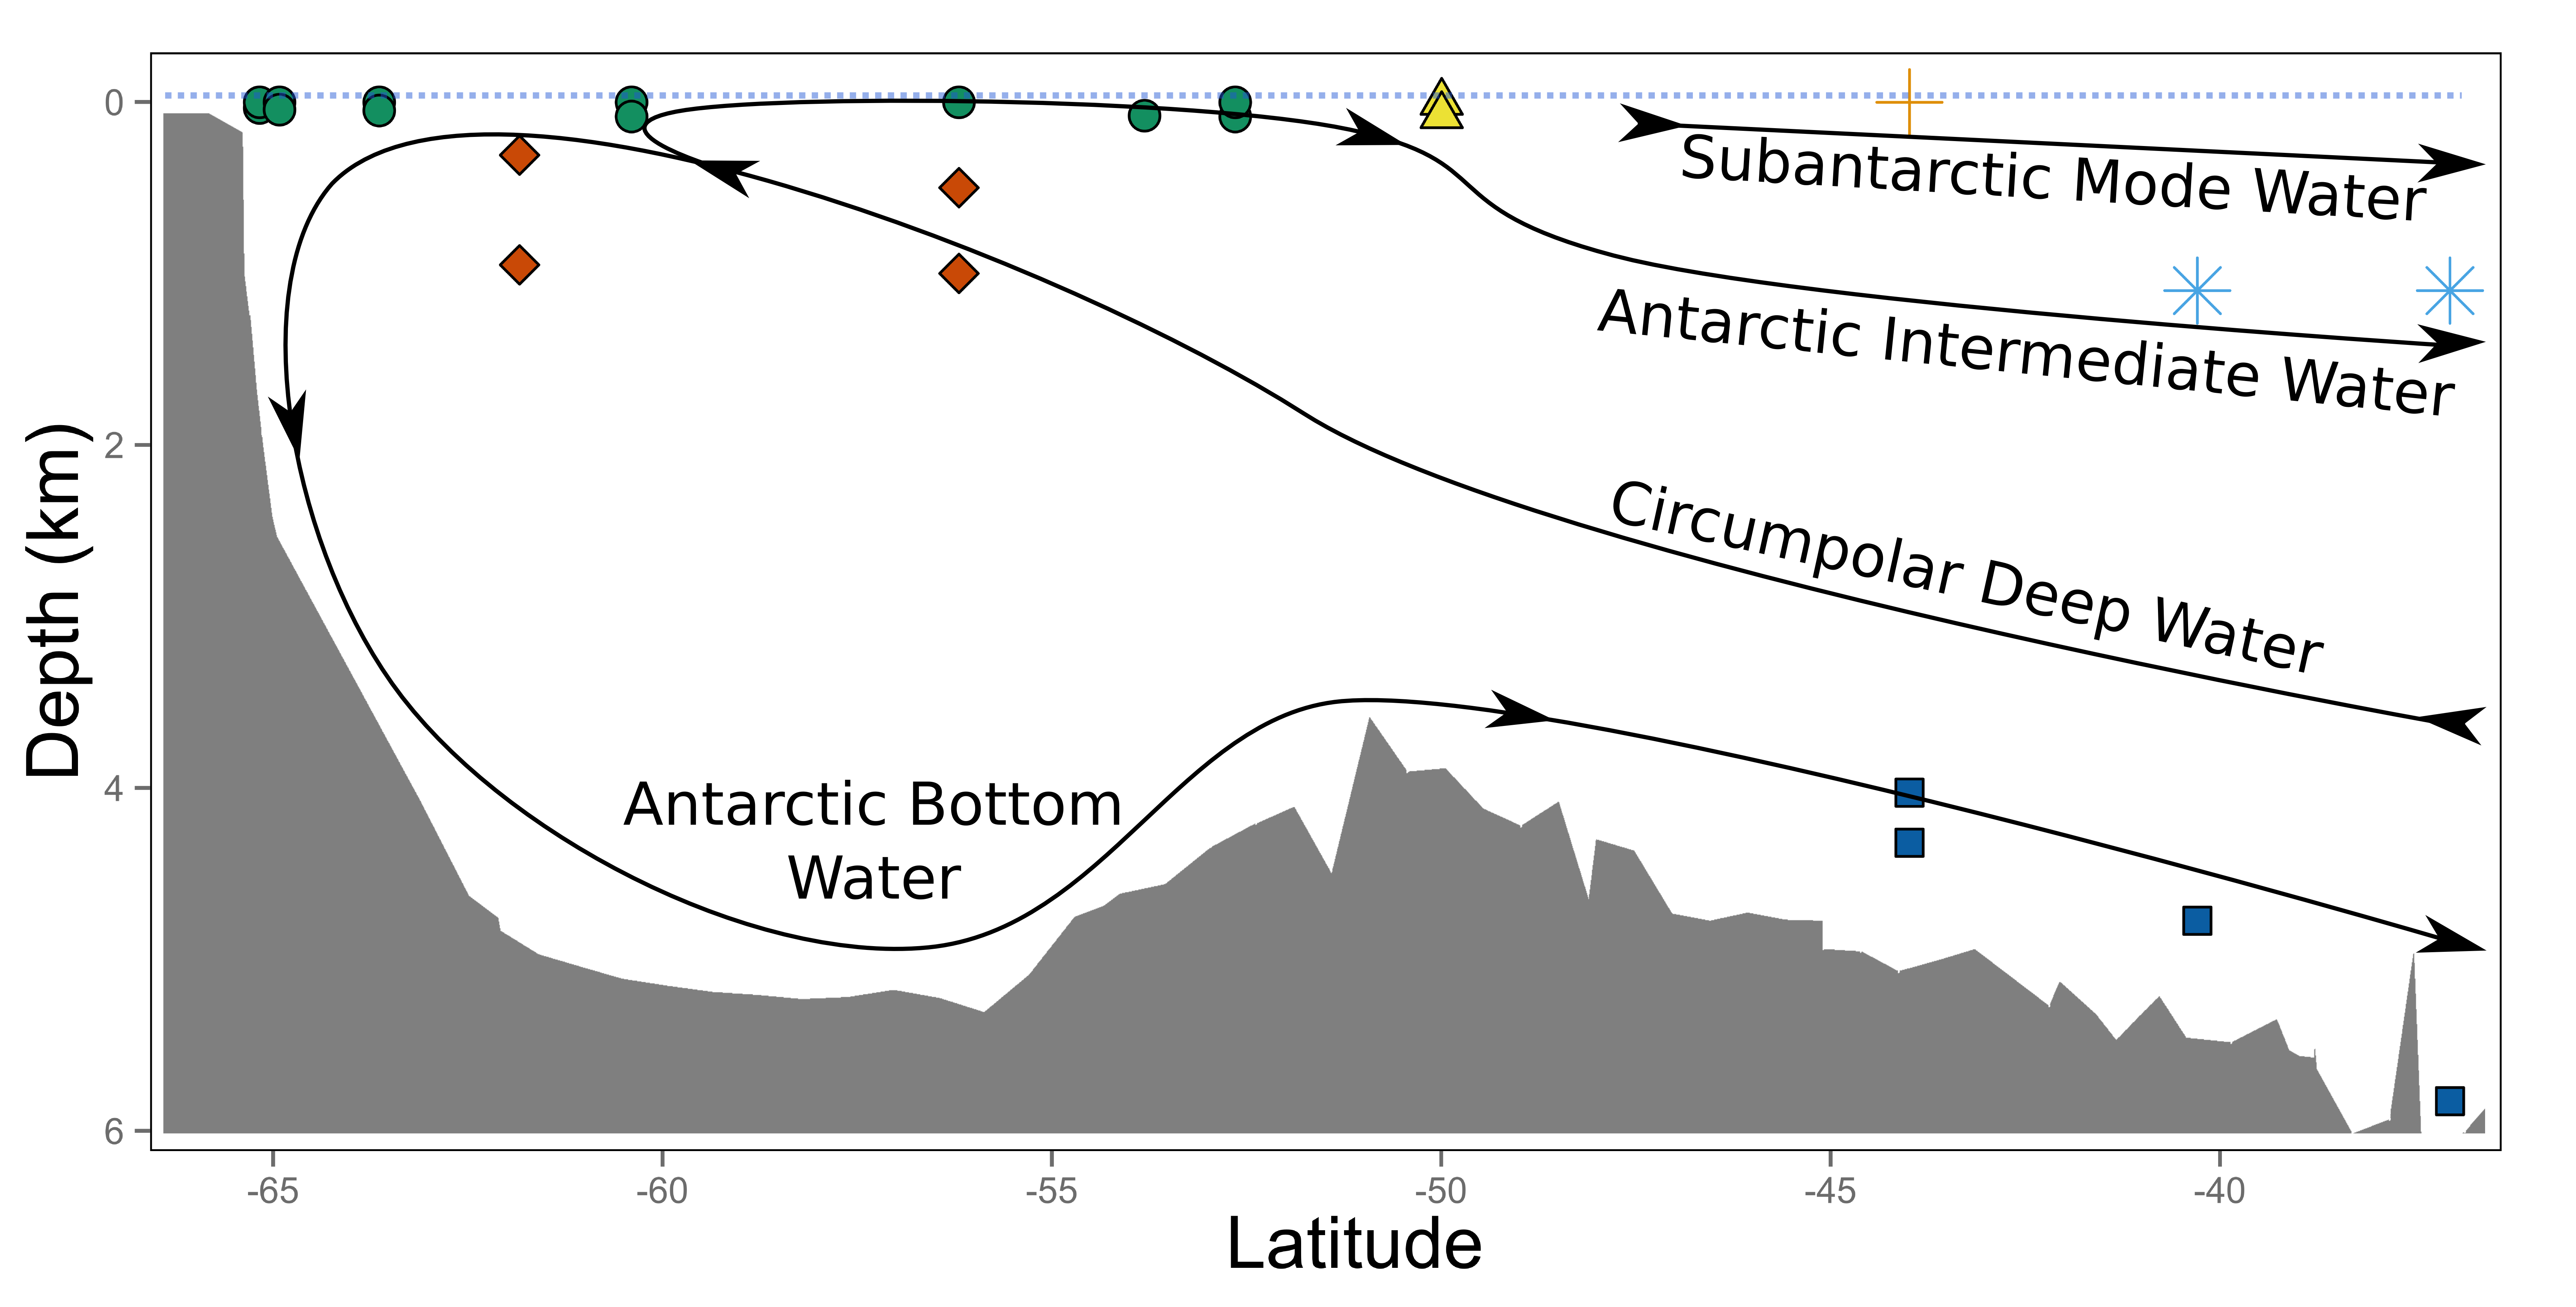
\includegraphics[width=\textwidth]{../advection/advectionsamplemap.png}
  \caption[Map showing sites of samples used in the advection study]{Antarctic Intermediate Waters (AAIW), light blue stars; Subantarctic Mode Water (SAMW), orange crosses; Antarctic Bottom Water (AABW), dark blue squares; Antarctic Zone (AZ), green circles; Polar Frontal Zone (PFZ), yellow triangles; Circumpolar Deep Water (CDW), red diamonds; sea surface, blue dashed horizontal line. Bathymetry is an approximate representation for 115\textdegree{} E, and is indicative only.}
  \label{fig:advectionsamplemap}
\end{figure}


Sampling\footnote{Sampling was performed by David Wilkins, Timothy J.\ Williams and Sheree Yau.} was conducted on board the RSV \textit{Aurora Australis} during cruise V3 from 20 January--7 February 2012.
This cruise occupied a latitudinal transect from waters north of Cape Poinsett, Antarctica (65\textdegree{} S) to south of Cape Leeuwin, Australia (37\textdegree{} S) within a longitudinal range of 113--115\textdegree{} E.

Sampling was performed as described in \secreft{ch:polarfront}, with sites and depths selected to provide coverage of all major \ac{SO} water masses.
At each surface station, \textapprox{}250--560 L of seawater was pumped from \textapprox{}1.5--2.5 m depth.
At some surface stations, an additional sample was taken from the \ac{DCM}, as determined by chlorophyll fluorescence measurements taken from a \ac{CTD} cast at each station.
Samples of mesopelagic and deeper waters (\textapprox{}120--240 L) were also collected at some stations using Niskin bottles attached to the \ac{CTD}.
Sampling depths were selected based on temperature, salinity and dissolved oxygen profiles to capture water from the targeted water masses.
Profiles were generated on the \ac{CTD} descent, and samples collected on the ascent at the selected depths.
Deep water masses were identified by the following criteria: \ac{CDW} = oxygen minimum (\ac{UCD}) or salinity maximum (\ac{LCD}); \ac{AABW} = deep potential temperature minimum; \ac{AAIW} = salinity minimum \cite{Foldvik:1988gp}.
Surface zones were identified relative to the major fronts of the \ac{SO}, which are marked by strong latitudinal gradients in temperature and salinity \cite{Sokolov:2002tc, Orsi:1995va}.
The \ac{AZ} lies south of the \ac{PF} (\textapprox{}51\textdegree{} S at the time of sampling), while the \ac{PFZ} lies between the \ac{PF} and the \ac{SAF}.
\ac{SAMW} overlays \ac{AAIW} north of the \ac{SAF}.
In total, 25 samples from the \ac{AZ}, \ac{PFZ}, \ac{SAMW}, \ac{AAIW}, \ac{CDW} and \ac{AABW} were collected for this study \figref{fig:advectionsamplemap}.

Seawater samples were prefiltered through a 20 \micron{} plankton net, then filtrate was captured on sequential 3.0 \micron{} 0.8 \micron{} and 0.1 \micron{} 293 mm polyethersulfone membrane filters (Pall, Port Washington, USA), and immediately stored at $-20$ $^\circ$C \cite{Rusch:2007ez,Ng:2010cd}.

\subsection{DNA extraction}

DNA extraction was performed using a modified version of the phenol-chloroform method described in \citet{Rusch:2007ez}.
Samples were thawed in a 37 \textdegree{}C water bath.
Half of the storage buffer (\textapprox{}10 mL) was decanted into a clean 50 mL centrifuge tube.
If the volume decanted was less than 10 mL, the difference was made with sterile water (Sigma-Aldrich, St.\ Louis, USA).
An equal volume of 50\% sucrose lysis buffer (50 mM TRIS-HCl, 40 mM EDTA, 0.75 M Sucrose, pH 8) was added such that the final concentration was 25\% sucrose lysis buffer.
A small pinch of lysozyme (Sigma-Aldrich, St.\ Louis, USA) (final concentration \textapprox{}2.5 mg/mL) and 1 mL TRIS-EDTA (10 mM TRIS, 1 mM EDTA, pH 8) was added.

The filter membrane was removed from the storage tube and cut in half aseptically.
One half was returned to the storage tube, which was refrozen at $-80$ \textdegree{}C.
The remaining half was cut in half again, and one quarter-filter placed atop the other such that the biomass (filtrand) on each piece was facing outwards.
Keeping the filters together, they were cut into very fine (\textapprox{}3 mm by 10 mm) strips, which were placed in the 50 mL centrifuge tube containing the buffer and lysozyme mixture.
This tube was mixed by gentle inversion, then tapped such that all filter strips collected at the bottom of the tube and were covered by lysis buffer.
The tube was then incubated in a 37 \textdegree{}C shaking water bath at 275 RPM for 30--60 min.

200 \microlitre{} of 20 mg/mL Proteinase K (Sigma-Aldrich, St.\ Louis, USA) was added to the tube, which was mixed by gentle inversion.
The tube was gently tapped such that all filter strips collected at the bottom covered by lysis buffer.
The tube was then subjected to three freeze-thaw cycles, each cycle consisting of 20--30 min in a $-80$ \textdegree{}C freezer followed by 20--30 min in a 55 \textdegree{}C water bath.
After the final complete thaw, 200 \microlitre{} of 20 mg/mL Proteinase K and 2 mL of 10\% SDS (Sigma-Aldrich, St.\ Louis, USA) were added to the tube.
The tube was mixed by gentle inversion then gently tapped such that all filter strips collected at the bottom covered by lysis buffer.
It was then incubated in a 55 \textdegree{}C shaking water bath at 175 RPM for two hours.

The supernatant was pipetted from the tube using a genomic tip and split evenly into two new 50 mL centrifuge tubes.
An equal volume of buffer-saturated (10 mM TRIS HCl, 1 mM EDTA, pH 8) phenol (Sigma-Aldrich, St.\ Louis, USA) was added to each of the tubes, which were mixed by gentle inversion.
The mixtures were then fractionated in a fixed-angle rotor centrifuge for 15 min at 3700 RPM at room temperature.
The bottom layer of each tube was removed by pipette into a new 50 mL centrifuge tube.
Each of these two tubes was then made to 50 mL with sterile water (Sigma-Aldrich, St.\ Louis, USA).
After mixing by gentle inversion, each 50 mL mixture was then split evenly into two new 50 mL centrifuge tubes, resulting in four tubes each containing 25 mL of mixture.
These tubes were then made to 50 mL with 1-propanol (Sigma-Aldrich, St.\ Louis, USA).
The mixtures were homogenised by gentle inversion and incubated at 4 \textdegree{}C overnight.

Following incubation, the tubes were centrifuged using a fixed-angle rotor for 30 min at 7500 RPM and room temperature.
The majority of the supernatant was removed by decanting, and the tubes left to sit until the remaining supernatant (\textapprox{}1 mL) collected at the bottom over the precipitated pellet.
The pellet was then resuspended by gentle pipetting with a genomic tip, and the suspension placed in a new 1.5 mL microcentrifuge tube (four tubes total).
These tubes were then centrifuged in a microcentrifuge for 10 minutes at 13,000 RPM and room temperature.
The supernatant was removed by pipette and the tubes placed in a 37 \textdegree{}C heat block with the lids opened and covered by a sterile KimWipe (Kimberly-Clark, Irving, USA) for 10 min, or longer if the supernatant did not evaporate completely in that time.
93.75 \microlitre{} of TRIS-EDTA was added to each tube, and the tubes were incubated at 4 \textdegree{}C for one hour to allow the DNA pellet to redissolve.

After this incubation, the pellets were gently pipetted with a genomic tip to ensure complete resuspension.
The suspensions from all four tubes were combined, and an additional 750 \microlitre{} of TRIS-EDTA added.
This was then split evenly into two new 1.5 mL microcentrifuge tubes (\textapprox{}562.5 \microlitre{} per tube).

750 \microlitre{} of buffer-saturated phenol was added to each tube, and the tubes mixed gently by inversion until a visible emulsion formed.
Phase separation was performed by centrifugation for 5 min at 13,000 RPM and room temperature.
The upper (aqueous) phase was removed to a new 1.5 mL microcentrifuge tube using a genomic tip.

750 \microlitre{} of phenol-chloroform-isoamyl alcohol (25:24:1) mixture (Sigma-Aldrich, St.\ Louis, USA) was added to each tube, and the tubes mixed by gentle inversion until a visible emulsion formed.
Phase separation was performed by centrifugation for 5 min at 13,000 RPM and room temperature.
The upper (aqueous) phase was removed to a new 1.5 mL microcentrifuge tube using a genomic tip.

75 \microlitre{} of 3 M sodium acetate (pH 8) and 750 \microlitre{} of 1-propanol was added to each tube.
The tubes were centrifuged at 13,000 RPM and room temperature for 30 min to precipitate the DNA.
The supernatant was removed by pipetting, and 100 \microlitre{} of 70\% ethanol added.
The tubes were centrifuged again at 13,000 RPM and room temperature for 5 min.
The supernatant was removed by pipetting and the DNA pellet dried in a 37 \textdegree{}C heat block.
The DNA was dissolved overnight in 40--200 \microlitre{} of TRIS-EDTA, depending on the expected yield.

\subsection{Sequencing}

Tag pyrosequencing was performed by Research and Testing Laboratory (Lubbock, USA) on a GS FLX+ platform (Roche, Branford, USA), using a modification of the standard 926F/1392R primers targeting the V6--V8 hypervariable regions of bacterial and archaeal 16S rRNA genes (926wF: \nsequence{AAA-CTY-AAA-KGA-ATT-GRC-GG}, 1392R: \nsequence{ACG-GGC-GGT-GTG-TRC}).
The additional wobble bases have been found to amplify a greater range of environmental bacteria and archaea, particularly Euryarchaeota, than the standard primers (Federico M.\ Lauro, personal communication).
Denoising, chimera removal and trimming of poor quality read ends were performed by the sequencing facility.

\subsection{Taxonomic assignment}

Using \ac{QIIME} 1.6.0 \cite{Caporaso:2010ts}, tag pyrosequencing reads were clustered at the 97\% sequence similarity level against the SILVA database of rRNA sequences (release 108, eukaryote and chloroplast sequences removed) \cite{Quast:2013hk}, with non-clustering reads discarded.
\ac{QIIME} was used to assign to each \ac{OTU} cluster a description representing the most detailed lineage common to at least 90\% of the clustered reads.
For ease of interpretation, full lineage descriptions were collapsed to the two most detailed ranks, with ranks labelled ``uncultured'' or ``other'' ignored.
To generate a taxonomic profile for each sample, the relative abundances of reads assigned to each \ac{OTU} in each size fraction were encoded as variables.
To account for the reads discarded during clustering, abundances in each size fraction were standardised by the proportion of reads retained from that fraction.
The abundances were square root transformed and Bray-Curtis dissimilarity indices between samples calculated in \softwarename{PRIMER 6} (PRIMER-E, Lutton, UK).

\subsection{Physicochemical and spatial distances}

Environmental data were collected from \ac{CTD} casts at each sample site.
Pressure, dissolved oxygen concentration and water temperature measurements were collected with \ac{CTD} instruments.
Salinity and concentrations of dissolved phosphate, nitrate and silicate were obtained from hydrochemical analysis of seawater samples collected in Niskin bottles during \ac{CTD} casts \cite{Rosenberg:2012vs}.
These samples were collected at discrete depths, and the hydrochemical sample closest to the depth of the relevant biological sample was selected.
The exceptions were samples 32 and 33 (49.5\textdegree{} S, 115\textdegree{} E), for which nitrate concentrations were not available, and sample 29 (53.2\textdegree{} S, 115\textdegree{} E) for which phosphate concentration was not available.
In these cases, a reading from the appropriate depth was substituted from the nearest available cast (50.0\textdegree{} S, 115\textdegree{} E for samples 32 and 33; 53.8\textdegree{} S, 115\textdegree{} E for sample 29).
Pressure values were $log(x+1)$ transformed to reduce right-skew \cite{Clarke:2011tn} and the combined instrument and hydrochemical data were used to create environmental profiles for each sample.
The variables were normalised and a Euclidean distance matrix generated in \softwarename{PRIMER 6}.

\ac{distLM} multivariate analysis \cite{Legendre:1999tj} was performed to confirm the selection of physicochemical variables and explore their relationship with taxonomic composition.
In \softwarename{PRIMER 6}, all possible combinations of variables (``BEST selection'') were explored by \ac{distLM}, and the models (sets of variables) that best fit the taxonomic dissimilarity matrix (adjusted R\textsuperscript{2} as the fitness measure) were selected.
The relationship between the resulting model and the taxonomic dissimilarity between samples was visualised by \ac{dbRDA} ordination.

To generate a spatial distance matrix, pairwise ellipsoidal distances between samples (including difference in depth) were calculated using \softwarename{INVERS3D} (National Oceanic and Atmospheric Administration, Silver Springs, USA).

\subsection{Generation of advection distance matrix}

In order to calculate advection distances between the sample sites, the release and advection of inertial particles was simulated using a computational model of \ac{SO} circulation\footnote{Modelling was performed by Erik van Sebille.}.
The circulation model used was the \ac{SOSE} \cite{Mazloff:2010et}, an eddy-permitting circulation model constrained by \textit{in situ} and satellite observations of the \ac{SO} during 2005-2006.
The \ac{CMS} \cite{Paris:2013fs} version 1.1 was used to calculate the three-dimensional trajectories of inertial particles in the \ac{SOSE} velocity fields using a Lagrangian toolset.
Three-dimensional velocity fields for the \ac{SO} from January 2005--December 2007 were simulated, and looped for 100 years as described in \citet{vanSebille:2012hh}.
The simulation had a temporal resolution of five days, and a spatial resolution of \nicefrac{1}{6}\textdegree{} of latitude and longitude and 42 levels of depth.
For each site, 100 particles were released every 5 days through the first loop of the simulation (total of 22,000 particles per site) at the latitude and depth of the site, evenly spaced along a 1\textdegree{} longitudinal line centred on the site longitudes.

The trajectory of each particle was analysed to detect encounters between particles and sample sites.
An encounter was defined as the vector between any two consecutive 5 day particle locations intersecting a box bounded by \textpm0.2\textdegree{} of latitude, \textpm0.5\textdegree{} of longitude and \textpm50 m of depth from a sample site.
A two-stage algorithm was designed to reduce the computational complexity of this analysis.
For each pair of consecutive (i.e.\ five-day) positions of each particle, the latitude, longitude and depth of each plane of each bounding box of each sample site was compared to the equivalent properties of the two positions.
For an intersection between the five-day vector of a particle and a sample bounding box to have occurred, at least one bounding box plane in at least one dimension must lie between the particle start and end position in that dimension.
This allowed five-day vectors which could not possibly have resulted in a collision to be quickly excluded.
The remaining vectors were then individually tested for intersections with the planes defining the bounding boxes for each sample using the \softwarename{perl} package \softwarename{math::zap}\footnote{Retrieved from \url{http://search.cpan.org/~prbrenan/Math-Zap-1.07/}.}.

Only the first encounter between any particle and sample was counted. Four pairs of samples (10/11; 12/13; 16/17; 21/22), where a \ac{DCM} sample was taken directly below a surface sample within the mixed layer, were too close to act as separate particle release sites.
For these samples, simulated particle releases were performed for only one of the pair, and the generated encounters were attributed to both. 
For all samples, the mean time in seconds between a particle being released from one sample and encountering another was calculated.
Pairwise advective distance between samples was defined as the mean of the two directional mean times between each sample in the pair.
This metric was selected to ensure advective flows which may be of high biological relevance, such as a small number of particles quickly transported between sites, were appropriately weighted when paired with flows of lower biological relevance, such as a large number of particles transported between sites over decades.
To ensure the results were robust to the choice of metric, subsequent statistical tests were repeated with pairwise advective distance redefined as the mean time for all pairwise encounters.
The pairwise distance between the surface/\ac{DCM} samples discussed above was set to zero.
For pairs of samples that did not yield mutual encounters (47 pairs, all including at least one \ac{AABW} sample; see Results), this was set to the maximum run time of the simulation (100 years).
Subsequent statistical tests were rerun with the \ac{DCM} and \ac{AABW} samples excluded to ensure these constraints were not unduly influencing the results (see ``Testing of advection effect'', below).

\subsection{Ordination of distance matrices and comparison to water masses}

Ordinations of the taxonomic, environmental and advection distance matrices were produced by \ac{nMDS} in \softwarename{PRIMER 6}.
\ac{ANOSIM} was also performed in \softwarename{PRIMER 6} to test for statistically significant differences between water masses in each of these three factors.
Right-tailed p-values for each test were computed using 999 random label permutations of one of the test matrices.

\subsection{Testing of advection effect}

Mantel tests were performed using \ac{PASSaGE 2} \cite{Rosenberg:2011uz}.
To test for and quantify distance and environment effects, partial Mantel tests were performed comparing the taxonomic matrix to the spatial then environmental matrices, with the remaining matrix held constant.
To test the hypothesis that advection shapes \ac{SO} microbial assemblages independent of distance and environment effects, a partial Mantel test was performed comparing the taxonomic and advection matrices, with both the spatial and environmental matrices held constant.
Right-tailed p-values for all tests were calculated using 999 random label permutations of one the test matrices.

To ensure that the result was not unduly influenced by the samples to which the 100 year ceiling was applied (all \ac{AABW}, see Results) and those for which particle releases were not simulated (samples 11, 13, 17 and 22), the test was repeated with these samples removed.

To confirm that the advection effect was directional, i.e.\ that ``upstream'' sites were acting as sources of diversity to ``downstream'' sites, \softwarename{SourceTracker} \cite{Knights:2011in} was used to identify sources of \acp{OTU} in each sample.
Each sample was sequentially designated a sink, with the remaining samples as potential sources, and the most probable proportion of \acp{OTU} originating from each potential source determined over 100 randomised trials per sample.
Spearman's rank correlation was then calculated between the \softwarename{SourceTracker} predicted source proportions and particle encounter source proportions for each sample pairwise, with right-tailed p-value determined by permutation.

\subsection{Differential influence of advection on OTU subsets}

It was hypothesised that some \acp{OTU} may be more amenable than others to advective dispersal: for example, cells able to form dormant states \cite{Bissett:2010wj}.
A modified form of the \softwarename{bvstep} algorithm \cite{Clarke:1998ki} was developed to investigate this.

\softwarename{bvstep} seeks to find a subset of a community of \acp{OTU}, the inter-sample resemblance pattern of which best matches that of the entire community.
The quality of the match is defined as the rank correlation (typically Spearman's \textrho) between the Bray-Curtis similarity matrix for the \ac{OTU} subset and that of the full set.
As the number of potential subsets grows exponentially with the number of \acp{OTU} ($2^{s}-1$ subsets for $s$ \acp{OTU} \cite{Clarke:1998ki}), it is computationally impractical to test each individually.
Hence, \softwarename{bvstep} uses a stepwise approach to efficiently explore the space of possible subsets.

The algorithm proceeds through successive rounds of forward and backward selection, beginning with a randomly selected subset of (typically six) \acp{OTU}.
In the forward selection round, each \ac{OTU} not currently in the subset is tested as a potential addition to the subset.
The \ac{OTU} that by its addition maximally increases the correlation of the subset to the full set is added to the subset, and forward selection is repeated.
If no \ac{OTU} can improve the current subset, forward selection in terminated and backward selection begins.

In the backward selection round, each \ac{OTU} currently in the subset is tested as a candidate for removal.
As with forward selection, the \ac{OTU} that by its removal maximally increases the correlation of the subset to the full set is removed, and backward selection is repeated.
If no such \ac{OTU} exists, backward selection is terminated and a new round of forward selection begins.
Successive rounds of forward and backward selection proceed until either the correlation exceeds 0.95, or no further increase in the correlation can be achieved by either forward or backward selection.

Typically, the algorithm will be run with multiple restarts, each with a randomly selected starting subset, and the resulting subsets compared.
This allows an estimation of the ``structural redundancy'' of the community: the number of unique, high-correlation subsets of \acp{OTU} which can be extracted from the total set without replacement.

The \softwarename{bvstep} implementation used in this study differs from the canonical version \cite{Clarke:1998ki} in two main ways.
Most significantly, each potential \ac{OTU} subset is not compared to the full set of \acp{OTU} by Spearman's rank correlation.
Instead, the Bray-Curtis resemblance matrix between samples is generated for each tested subset, and compared to the advection distance matrix using a partial Mantel test holding the spatial and environmental distances constant.
This modified form of the algorithm thus addressed the question of whether some subset of \acp{OTU} were as (or more) affected by advection as the entire set.
Unlike the standard algorithm, where the best possible ``subset'' is simply the full set of samples (\textrho{} = 1), with this modified algorithm it is possible for a subset to yield a better correlation than the full set.

Additionally, after the random selection of six \acp{OTU} to form the starting subset, only the single \ac{OTU} with the highest correlation is retained.
This was because it was observed that the starting subset of \acp{OTU} were very rarely retained through the entire selection process, presumably because the total number of \acp{OTU} was high and the random selection of representative \acp{OTU} thus unlikely.
Removing five of the starting \acp{OTU} immediately thus eliminates many unnecessary rounds of selection.

\section{Results}

\subsection{Sequencing and taxonomic assignment}

After trimming, denoising and chimera removal, the 25 samples (each with three separately sequenced size fractions) yielded 1,008,963 pyrosequencing reads of length 251--561 bp (mean 426 bp).
Individual fractions yielded 3,687--52,192 reads (mean 13,453).
After clustering against the SILVA database, 2,295--30,760 (mean 9,618) reads per fraction were retained for taxonomic assignment.

1417 unique \acp{OTU} were identified across all fractions of all samples.
The Chao 1 statistic was calculated, and estimated \ac{OTU} were under-sequenced by 0--50\% across all samples (mean 26\%) \tabref{tab:advectionfullsampledata}.
In all water masses, decreasing numbers of reads yielded \ac{OTU} assignments as size fraction increased \figref{fig:taxonomicbarplot}.
This probably reflects an increasing number of eukaryotic cells (which were excluded from \ac{OTU} assignment) on the higher fractions.
A full list of \ac{OTU} assigments and relative abundances is given in the supplementary material \suppfile{advection-all-OTUs.txt}.

{\footnotesize \sffamily
\begin{landscape}
\begin{longtable}{llllllllllllllll}
\caption[Full sample data for advection study]{\sffamily{}Full location, summary of taxonomic assignments and full physicochemical data for each of the 25 samples in this study. Units are given in column headers. Water mass abbreviations are Antarctic Intermediate Waters (AAIW); Subantarctic Mode Water (SAMW); Antarctic Bottom Water (AABW); Antarctic Zone (AZ); Polar Frontal Zone (PFZ); Circumpolar Deep Water (CDW).} 
\\
\toprule
\textbf{Sample} & \textbf{Fraction} & \textbf{Date} & \textbf{Lat.} & \textbf{Lon.} & \textbf{Depth} & \textbf{Water} & \textbf{OTU} & \textbf{Chao 1} & \textbf{Pressure} & \textbf{Oxygen} & \textbf{Temperature} & \textbf{Phosphate} & \textbf{Nitrate} & \textbf{Silicate} & \textbf{Salinity}\\
& \textbf{(\micron)} & & (\textdegree{}) & (\textdegree{}) & \textbf{(m)} & \textbf{mass} & \textbf{count} & & \textbf{(dbar)} & \textbf{(\textmu{}mol/L)} & \textbf{(\textdegree{}C)} & \textbf{(\textmu{}mol/L)} & \textbf{(\textmu{}mol/L)} & \textbf{(\textmu{}mol/L)} & \textbf{(PSU)}\\
\midrule \endfirsthead
\caption{(cont.) Full sample data for advection study.}
\\
\toprule
\textbf{Sample} & \textbf{Fraction} & \textbf{Date} & \textbf{Lat.} & \textbf{Lon.} & \textbf{Depth} & \textbf{Water} & \textbf{OTU} & \textbf{Chao 1} & \textbf{Pressure} & \textbf{Oxygen} & \textbf{Temperature} & \textbf{Phosphate} & \textbf{Nitrate} & \textbf{Silicate} & \textbf{Salinity}\\
& \textbf{(\micron)} & & (\textdegree{}) & (\textdegree{}) & \textbf{(m)} & \textbf{mass} & \textbf{count} & & \textbf{(dbar)} & \textbf{(\textmu{}mol/L)} & \textbf{(\textdegree{}C)} & \textbf{(\textmu{}mol/L)} & \textbf{(\textmu{}mol/L)} & \textbf{(\textmu{}mol/L)} & \textbf{(PSU)}\\
\midrule \endhead
\bottomrule 
\multicolumn{16}{l}{\textbf{\scriptsize{Continued on following page.}}}\\
\endfoot \endlastfoot
10 & 0.1 & 20/01/2012 & \textminus{}65.17 & 113.1 & 35 & AZ & 431 & 570 & 36 & 348.1 & \textminus{}1.125 & 1.82 & 26.73 & 60.6 & 33.6\\
10 & 0.8 & 20/01/2012 & \textminus{}65.17 & 113.1 & 35 & AZ & 444 & 593 & 36 & 348.1 & \textminus{}1.125 & 1.82 & 26.73 & 60.6 & 33.6\\
10 & 3.0 & 20/01/2012 & \textminus{}65.17 & 113.1 & 35 & AZ & 148 & 293 & 36 & 348.1 & \textminus{}1.125 & 1.82 & 26.73 & 60.6 & 33.6\\
11 & 0.1 & 20/01/2012 & \textminus{}65.17 & 113.1 & 2 & AZ & 433 & 655 & 2 & 365.7 & \textminus{}0.798 & 1.66 & 25.13 & 57.8 & 33.4\\
11 & 0.8 & 20/01/2012 & \textminus{}65.17 & 113.1 & 2 & AZ & 241 & 422 & 2 & 365.7 & \textminus{}0.798 & 1.66 & 25.13 & 57.8 & 33.4\\
11 & 3.0 & 20/01/2012 & \textminus{}65.17 & 113.1 & 2 & AZ & 145 & 202 & 2 & 365.7 & \textminus{}0.798 & 1.66 & 25.13 & 57.8 & 33.4\\
12 & 0.1 & 21/01/2012 & \textminus{}64.92 & 113.3 & 2 & AZ & 294 & 387 & 2 & 356.4 & \textminus{}0.358 & 1.70 & 25.87 & 55.0 & 33.7\\
12 & 0.8 & 21/01/2012 & \textminus{}64.92 & 113.3 & 2 & AZ & 68 & 79 & 2 & 356.4 & \textminus{}0.358 & 1.70 & 25.87 & 55.0 & 33.7\\
12 & 3.0 & 21/01/2012 & \textminus{}64.92 & 113.3 & 2 & AZ & 158 & 232 & 2 & 356.4 & \textminus{}0.358 & 1.70 & 25.87 & 55.0 & 33.7\\
13 & 0.1 & 21/01/2012 & \textminus{}64.92 & 113.3 & 45 & AZ & 259 & 363 & 46 & 314.9 & \textminus{}1.604 & 2.05 & 30.17 & 65.8 & 34.2\\
13 & 0.8 & 21/01/2012 & \textminus{}64.92 & 113.3 & 45 & AZ & 299 & 418 & 46 & 314.9 & \textminus{}1.604 & 2.05 & 30.17 & 65.8 & 34.2\\
13 & 3.0 & 21/01/2012 & \textminus{}64.92 & 113.3 & 45 & AZ & 115 & 160 & 46 & 314.9 & \textminus{}1.604 & 2.05 & 30.17 & 65.8 & 34.2\\
16 & 0.1 & 22/01/2012 & \textminus{}63.64 & 113.3 & 2 & AZ & 245 & 338 & 2 & 355.9 & 0.500 & 1.62 & 24.60 & 47.1 & 33.8\\
16 & 0.8 & 22/01/2012 & \textminus{}63.64 & 113.3 & 2 & AZ & 210 & 307 & 2 & 355.9 & 0.500 & 1.62 & 24.60 & 47.1 & 33.8\\
16 & 3.0 & 22/01/2012 & \textminus{}63.64 & 113.3 & 2 & AZ & 135 & 222 & 2 & 355.9 & 0.500 & 1.62 & 24.60 & 47.1 & 33.8\\
17 & 0.1 & 22/01/2012 & \textminus{}63.64 & 113.3 & 50 & AZ & 169 & 219 & 50 & 319.1 & \textminus{}1.352 & 2.06 & 29.69 & 63.3 & 34.2\\
17 & 0.8 & 22/01/2012 & \textminus{}63.64 & 113.3 & 50 & AZ & 227 & 315 & 50 & 319.1 & \textminus{}1.352 & 2.06 & 29.69 & 63.3 & 34.2\\
17 & 3.0 & 22/01/2012 & \textminus{}63.64 & 113.3 & 50 & AZ & 199 & 290 & 50 & 319.1 & \textminus{}1.352 & 2.06 & 29.69 & 63.3 & 34.2\\
18 & 0.1 & 24/01/2012 & \textminus{}61.84 & 113.5 & 310 & CDW & 474 & 666 & 314 & 186.8 & 1.909 & 2.35 & 34.09 & 83.2 & 34.6\\
18 & 0.8 & 24/01/2012 & \textminus{}61.84 & 113.5 & 310 & CDW & 466 & 676 & 314 & 186.8 & 1.909 & 2.35 & 34.09 & 83.2 & 34.6\\
18 & 3.0 & 24/01/2012 & \textminus{}61.84 & 113.5 & 310 & CDW & 136 & 172 & 314 & 186.8 & 1.909 & 2.35 & 34.09 & 83.2 & 34.6\\
19 & 0.1 & 24/01/2012 & \textminus{}61.84 & 113.5 & 950 & CDW & 138 & 205 & 962 & 202.4 & 1.624 & 2.18 & 31.59 & 95.1 & 34.7\\
19 & 0.8 & 24/01/2012 & \textminus{}61.84 & 113.5 & 950 & CDW & 124 & 153 & 962 & 202.4 & 1.624 & 2.18 & 31.59 & 95.1 & 34.7\\
19 & 3.0 & 24/01/2012 & \textminus{}61.84 & 113.5 & 950 & CDW & 214 & 315 & 962 & 202.4 & 1.624 & 2.18 & 31.59 & 95.1 & 34.7\\
21 & 0.1 & 25/01/2012 & \textminus{}60.40 & 115.0 & 2 & AZ & 287 & 385 & 2 & 335.8 & 2.462 & 1.75 & 26.62 & 16.2 & 33.9\\
21 & 0.8 & 25/01/2012 & \textminus{}60.40 & 115.0 & 2 & AZ & 217 & 296 & 2 & 335.8 & 2.462 & 1.75 & 26.62 & 16.2 & 33.9\\
21 & 3.0 & 25/01/2012 & \textminus{}60.40 & 115.0 & 2 & AZ & 153 & 240 & 2 & 335.8 & 2.462 & 1.75 & 26.62 & 16.2 & 33.9\\
22 & 0.1 & 25/01/2012 & \textminus{}60.40 & 115.0 & 85 & AZ & 318 & 458 & 86 & 336.4 & 1.724 & 1.96 & 28.52 & 24.7 & 33.9\\
22 & 0.8 & 25/01/2012 & \textminus{}60.40 & 115.0 & 85 & AZ & 298 & 418 & 86 & 336.4 & 1.724 & 1.96 & 28.52 & 24.7 & 33.9\\
22 & 3.0 & 25/01/2012 & \textminus{}60.40 & 115.0 & 85 & AZ & 323 & 420 & 86 & 336.4 & 1.724 & 1.96 & 28.52 & 24.7 & 33.9\\
25 & 0.1 & 27/01/2012 & \textminus{}56.19 & 115.0 & 500 & CDW & 297 & 423 & 506 & 187.7 & 2.296 & 2.39 & 35.09 & 72.9 & 34.5\\
25 & 0.8 & 27/01/2012 & \textminus{}56.19 & 115.0 & 500 & CDW & 595 & 736 & 506 & 187.7 & 2.296 & 2.39 & 35.09 & 72.9 & 34.5\\
25 & 3.0 & 27/01/2012 & \textminus{}56.19 & 115.0 & 500 & CDW & 307 & 396 & 506 & 187.7 & 2.296 & 2.39 & 35.09 & 72.9 & 34.5\\
26 & 0.1 & 27/01/2012 & \textminus{}56.19 & 115.0 & 1000 & CDW & 257 & 316 & 1012 & 190.1 & 2.107 & 2.23 & 32.90 & 80.7 & 34.7\\
26 & 0.8 & 27/01/2012 & \textminus{}56.19 & 115.0 & 1000 & CDW & 438 & 510 & 1012 & 190.1 & 2.107 & 2.23 & 32.90 & 80.7 & 34.7\\
26 & 3.0 & 27/01/2012 & \textminus{}56.19 & 115.0 & 1000 & CDW & 380 & 584 & 1012 & 190.1 & 2.107 & 2.23 & 32.90 & 80.7 & 34.7\\
27 & 0.1 & 27/01/2012 & \textminus{}56.19 & 115.0 & 2 & AZ & 368 & 491 & 2 & 324.8 & 4.159 & 1.64 & 25.32 & 9.60 & 33.8\\
27 & 0.8 & 27/01/2012 & \textminus{}56.19 & 115.0 & 2 & AZ & 318 & 454 & 2 & 324.8 & 4.159 & 1.64 & 25.32 & 9.60 & 33.8\\
27 & 3.0 & 27/01/2012 & \textminus{}56.19 & 115.0 & 2 & AZ & 288 & 394 & 2 & 324.8 & 4.159 & 1.64 & 25.32 & 9.60 & 33.8\\
29 & 0.1 & 28/01/2012 & \textminus{}53.81 & 115.0 & 80 & AZ & 281 & 394 & 80 & 324.4 & 4.399 & 1.66 & 24.78 & 7.80 & 33.8\\
29 & 0.8 & 28/01/2012 & \textminus{}53.81 & 115.0 & 80 & AZ & 261 & 377 & 80 & 324.4 & 4.399 & 1.66 & 24.78 & 7.80 & 33.8\\
29 & 3.0 & 28/01/2012 & \textminus{}53.81 & 115.0 & 80 & AZ & 271 & 403 & 80 & 324.4 & 4.399 & 1.66 & 24.78 & 7.80 & 33.8\\
30 & 0.1 & 29/01/2012 & \textminus{}52.65 & 115.0 & 85 & AZ & 217 & 341 & 86 & 330.8 & 3.517 & 1.73 & 26.27 & 15.7 & 33.8\\
30 & 0.8 & 29/01/2012 & \textminus{}52.65 & 115.0 & 85 & AZ & 244 & 358 & 86 & 330.8 & 3.517 & 1.73 & 26.27 & 15.7 & 33.8\\
30 & 3.0 & 29/01/2012 & \textminus{}52.65 & 115.0 & 85 & AZ & 269 & 393 & 86 & 330.8 & 3.517 & 1.73 & 26.27 & 15.7 & 33.8\\
31 & 0.1 & 29/01/2012 & \textminus{}52.65 & 115.0 & 2 & AZ & 392 & 486 & 2 & 332.2 & 3.941 & 1.70 & 26.15 & 15.4 & 33.8\\
31 & 0.8 & 29/01/2012 & \textminus{}52.65 & 115.0 & 2 & AZ & 317 & 470 & 2 & 332.2 & 3.941 & 1.70 & 26.15 & 15.4 & 33.8\\
31 & 3.0 & 29/01/2012 & \textminus{}52.65 & 115.0 & 2 & AZ & 332 & 425 & 2 & 332.2 & 3.941 & 1.70 & 26.15 & 15.4 & 33.8\\
32 & 0.1 & 30/01/2012 & \textminus{}49.99 & 115.0 & 2 & PFZ & 297 & 407 & 2 & 306.9 & 7.412 & 1.40 & 22.74 & 4.00 & 33.9\\
32 & 0.8 & 30/01/2012 & \textminus{}49.99 & 115.0 & 2 & PFZ & 269 & 337 & 2 & 306.9 & 7.412 & 1.40 & 22.74 & 4.00 & 33.9\\
32 & 3.0 & 30/01/2012 & \textminus{}49.99 & 115.0 & 2 & PFZ & 225 & 304 & 2 & 306.9 & 7.412 & 1.40 & 22.74 & 4.00 & 33.9\\
33 & 0.1 & 30/01/2012 & \textminus{}49.99 & 115.0 & 80 & PFZ & 325 & 422 & 80 & 300.3 & 7.061 & 1.39 & 23.02 & 4.20 & 34.0\\
33 & 0.8 & 30/01/2012 & \textminus{}49.99 & 115.0 & 80 & PFZ & 352 & 547 & 80 & 300.3 & 7.061 & 1.39 & 23.02 & 4.20 & 34.0\\
33 & 3.0 & 30/01/2012 & \textminus{}49.99 & 115.0 & 80 & PFZ & 326 & 473 & 80 & 300.3 & 7.061 & 1.39 & 23.02 & 4.20 & 34.0\\
38 & 0.1 & 03/02/2012 & \textminus{}43.99 & 115.0 & 2 & SAMW & 383 & 494 & 2 & 279.1 & 13.02 & 0.59 & 4.540 & 1.40 & 34.7\\
38 & 0.8 & 03/02/2012 & \textminus{}43.99 & 115.0 & 2 & SAMW & 215 & 220 & 2 & 279.1 & 13.02 & 0.59 & 4.540 & 1.40 & 34.7\\
38 & 3.0 & 03/02/2012 & \textminus{}43.99 & 115.0 & 2 & SAMW & 177 & 181 & 2 & 279.1 & 13.02 & 0.59 & 4.540 & 1.40 & 34.7\\
39 & 0.1 & 03/02/2012 & \textminus{}43.99 & 115.0 & 4320 & AABW & 520 & 682 & 4400 & 217.5 & 0.8497 & 2.30 & 32.92 & 127 & 34.7\\
39 & 0.8 & 03/02/2012 & \textminus{}43.99 & 115.0 & 4320 & AABW & 158 & 215 & 4400 & 217.5 & 0.8497 & 2.30 & 32.92 & 127 & 34.7\\
39 & 3.0 & 03/02/2012 & \textminus{}43.99 & 115.0 & 4320 & AABW & 129 & 152 & 4400 & 217.5 & 0.8497 & 2.30 & 32.92 & 127 & 34.7\\
40 & 0.1 & 03/02/2012 & \textminus{}43.99 & 115.0 & 4028 & AABW & 77 & 102 & 4100 & 216.9 & 0.8503 & 2.29 & 32.94 & 126 & 34.7\\
40 & 0.8 & 03/02/2012 & \textminus{}43.99 & 115.0 & 4028 & AABW & 156 & 203 & 4100 & 216.9 & 0.8503 & 2.29 & 32.94 & 126 & 34.7\\
40 & 3.0 & 03/02/2012 & \textminus{}43.99 & 115.0 & 4028 & AABW & 42 & 48 & 4100 & 216.9 & 0.8503 & 2.29 & 32.94 & 126 & 34.7\\
44 & 0.1 & 05/02/2012 & \textminus{}40.29 & 115.0 & 4775 & AABW & 248 & 303 & 4866 & 217.9 & 0.8716 & 2.28 & 33.15 & 130 & 34.7\\
44 & 0.8 & 05/02/2012 & \textminus{}40.29 & 115.0 & 4775 & AABW & 405 & 497 & 4866 & 217.9 & 0.8716 & 2.28 & 33.15 & 130 & 34.7\\
44 & 3.0 & 05/02/2012 & \textminus{}40.29 & 115.0 & 4775 & AABW & 370 & 442 & 4866 & 217.9 & 0.8716 & 2.28 & 33.15 & 130 & 34.7\\
45 & 0.1 & 05/02/2012 & \textminus{}40.29 & 115.0 & 1100 & AAIW & 601 & 779 & 1112 & 199.4 & 4.321 & 2.12 & 31.29 & 33.9 & 34.4\\
45 & 0.8 & 05/02/2012 & \textminus{}40.29 & 115.0 & 1100 & AAIW & 150 & 151 & 1112 & 199.4 & 4.321 & 2.12 & 31.29 & 33.9 & 34.4\\
45 & 3.0 & 05/02/2012 & \textminus{}40.29 & 115.0 & 1100 & AAIW & 118 & 124 & 1112 & 199.4 & 4.321 & 2.12 & 31.29 & 33.9 & 34.4\\
46 & 0.1 & 07/02/2012 & \textminus{}37.05 & 115.0 & 1100 & AAIW & 166 & 176 & 1112 & 201.7 & 5.233 & 2.20 & 32.12 & 39.5 & 34.4\\
46 & 0.8 & 07/02/2012 & \textminus{}37.05 & 115.0 & 1100 & AAIW & 227 & 312 & 1112 & 201.7 & 5.233 & 2.20 & 32.12 & 39.5 & 34.4\\
46 & 3.0 & 07/02/2012 & \textminus{}37.05 & 115.0 & 1100 & AAIW & 251 & 360 & 1112 & 201.7 & 5.233 & 2.20 & 32.12 & 39.5 & 34.4\\
47 & 0.1 & 07/02/2012 & \textminus{}37.05 & 115.0 & 5827 & AABW & 138 & 248 & 5952 & 217.2 & 1.030 & 2.29 & 33.00 & 129 & 34.7\\
47 & 0.8 & 07/02/2012 & \textminus{}37.05 & 115.0 & 5827 & AABW & 379 & 509 & 5952 & 217.2 & 1.030 & 2.29 & 33.00 & 129 & 34.7\\
47 & 3.0 & 07/02/2012 & \textminus{}37.05 & 115.0 & 5827 & AABW & 106 & 123 & 5952 & 217.2 & 1.030 & 2.29 & 33.00 & 129 & 34.7\\
\bottomrule
\label{tab:advectionfullsampledata}
\end{longtable}
\end{landscape}
}

\begin{figure}[!ht]
  \centering
  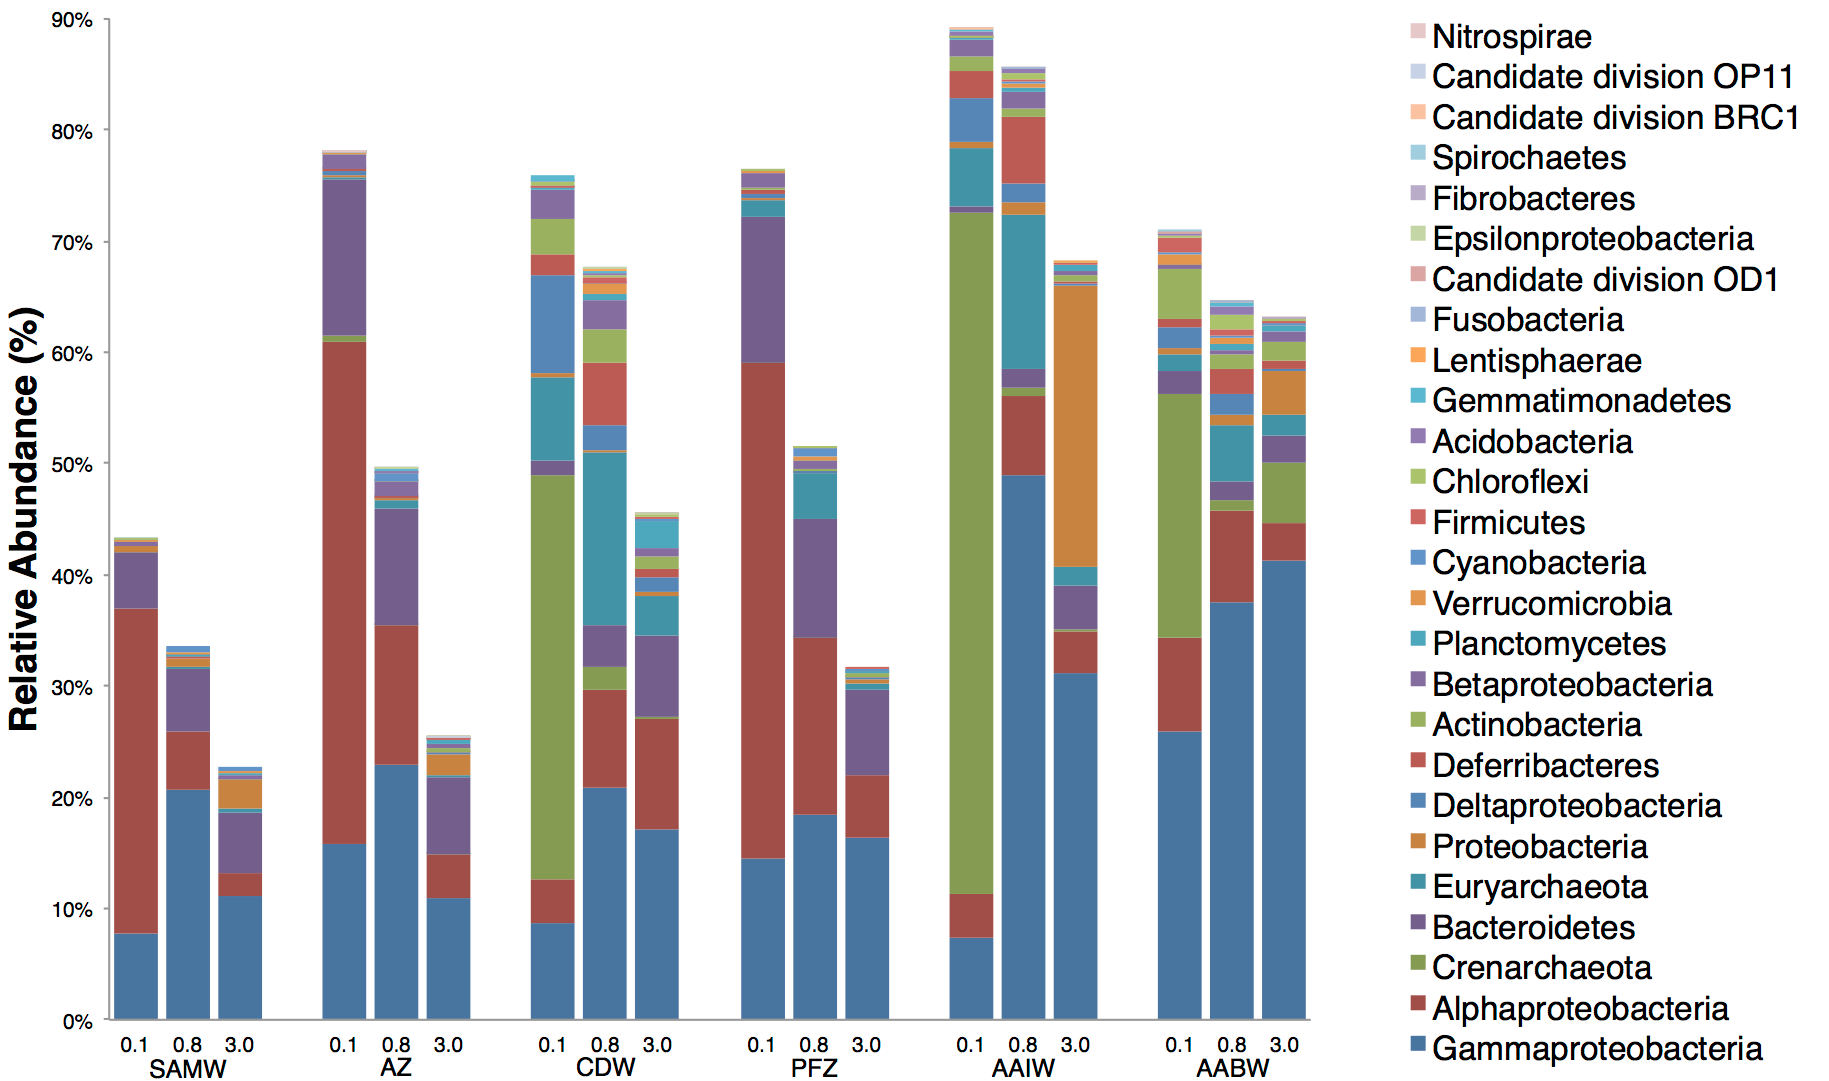
\includegraphics[width=\textwidth]{../advection/taxonomicbarplot.png}
  \caption[OTU assignments in the advection study.]{Taxonomic assignments for each sampled water mass. Water masses (x-axis): Subantarctic Mode Water (SAMW); Antarctic Zone (AZ); Circumpolar Deep Water (CDW); Polar Frontal Zone (PFZ); Antarctic Intermediate Water (AAIW); Antarctic Bottom Water (AABW). Size fractions are given in \micron{}. All \acp{OTU} aggregated to phylum, except for members of the Proteobacteria which were aggregated to class when known. Relative abundance is percentage of all reads assigned to a given taxonomic group and has been scaled to account for unassigned reads.}
  \label{fig:taxonomicbarplot}
\end{figure}


\ac{nMDS} ordination showed that the sampled water masses could be distinguished on the basis of taxonomic distance \figref{fig:nMDStaxonomic}.
This was supported by \ac{ANOSIM} analysis (R = 0.77, p = 0.001).
While each water mass had a distinct taxonomic profile, some broad differences between surface and deep masses were observed \figref{fig:taxonomicbarplot}.
Surface waters (\ac{AZ}, \ac{PFZ}, \ac{SAMW}) were dominated by representatives of the Alphaproteobacteria, Bacteroidetes and Gammaproteobacteria.
The high abundance of Bacteroidetes at the surface reflects their association with phytoplankton, as many species in this lineage specialise in the degradation of high molecular weight products of primary production \cite{Williams:2012gsa}.
Alphaproteobacteria were represented primarily by the SAR11 clade, abundant in ocean surface communities \cite{Morris:2002bn} including the \ac{SO} \cite{Brown:2012gna}, and Roseobacter clades, which have also been associated with degradation of phytoplankton products \cite{Williams:2012gsa, Giebel:2009hr}.
The dominant Gammaproteobacterial orders were the Alteromonadales and Oceanospirillales, typical of \ac{SO} surface waters \cite{Wilkins:2012ii}.
Few archaeal \acp{OTU} were detected, consistent with their well-described decline in abundance during summer \cite{Murray:1998wy, Grzymski:2012ej}.
The deep water masses (\ac{CDW}, \ac{AAIW}, \ac{AABW}) were dominated by Crenarchaeota, Euryarchaeota and Gammaproteobacteria, again consistent with previous findings \cite{LopezGarcia:2001vp}.

\begin{figure}[!ht]
  \centering
  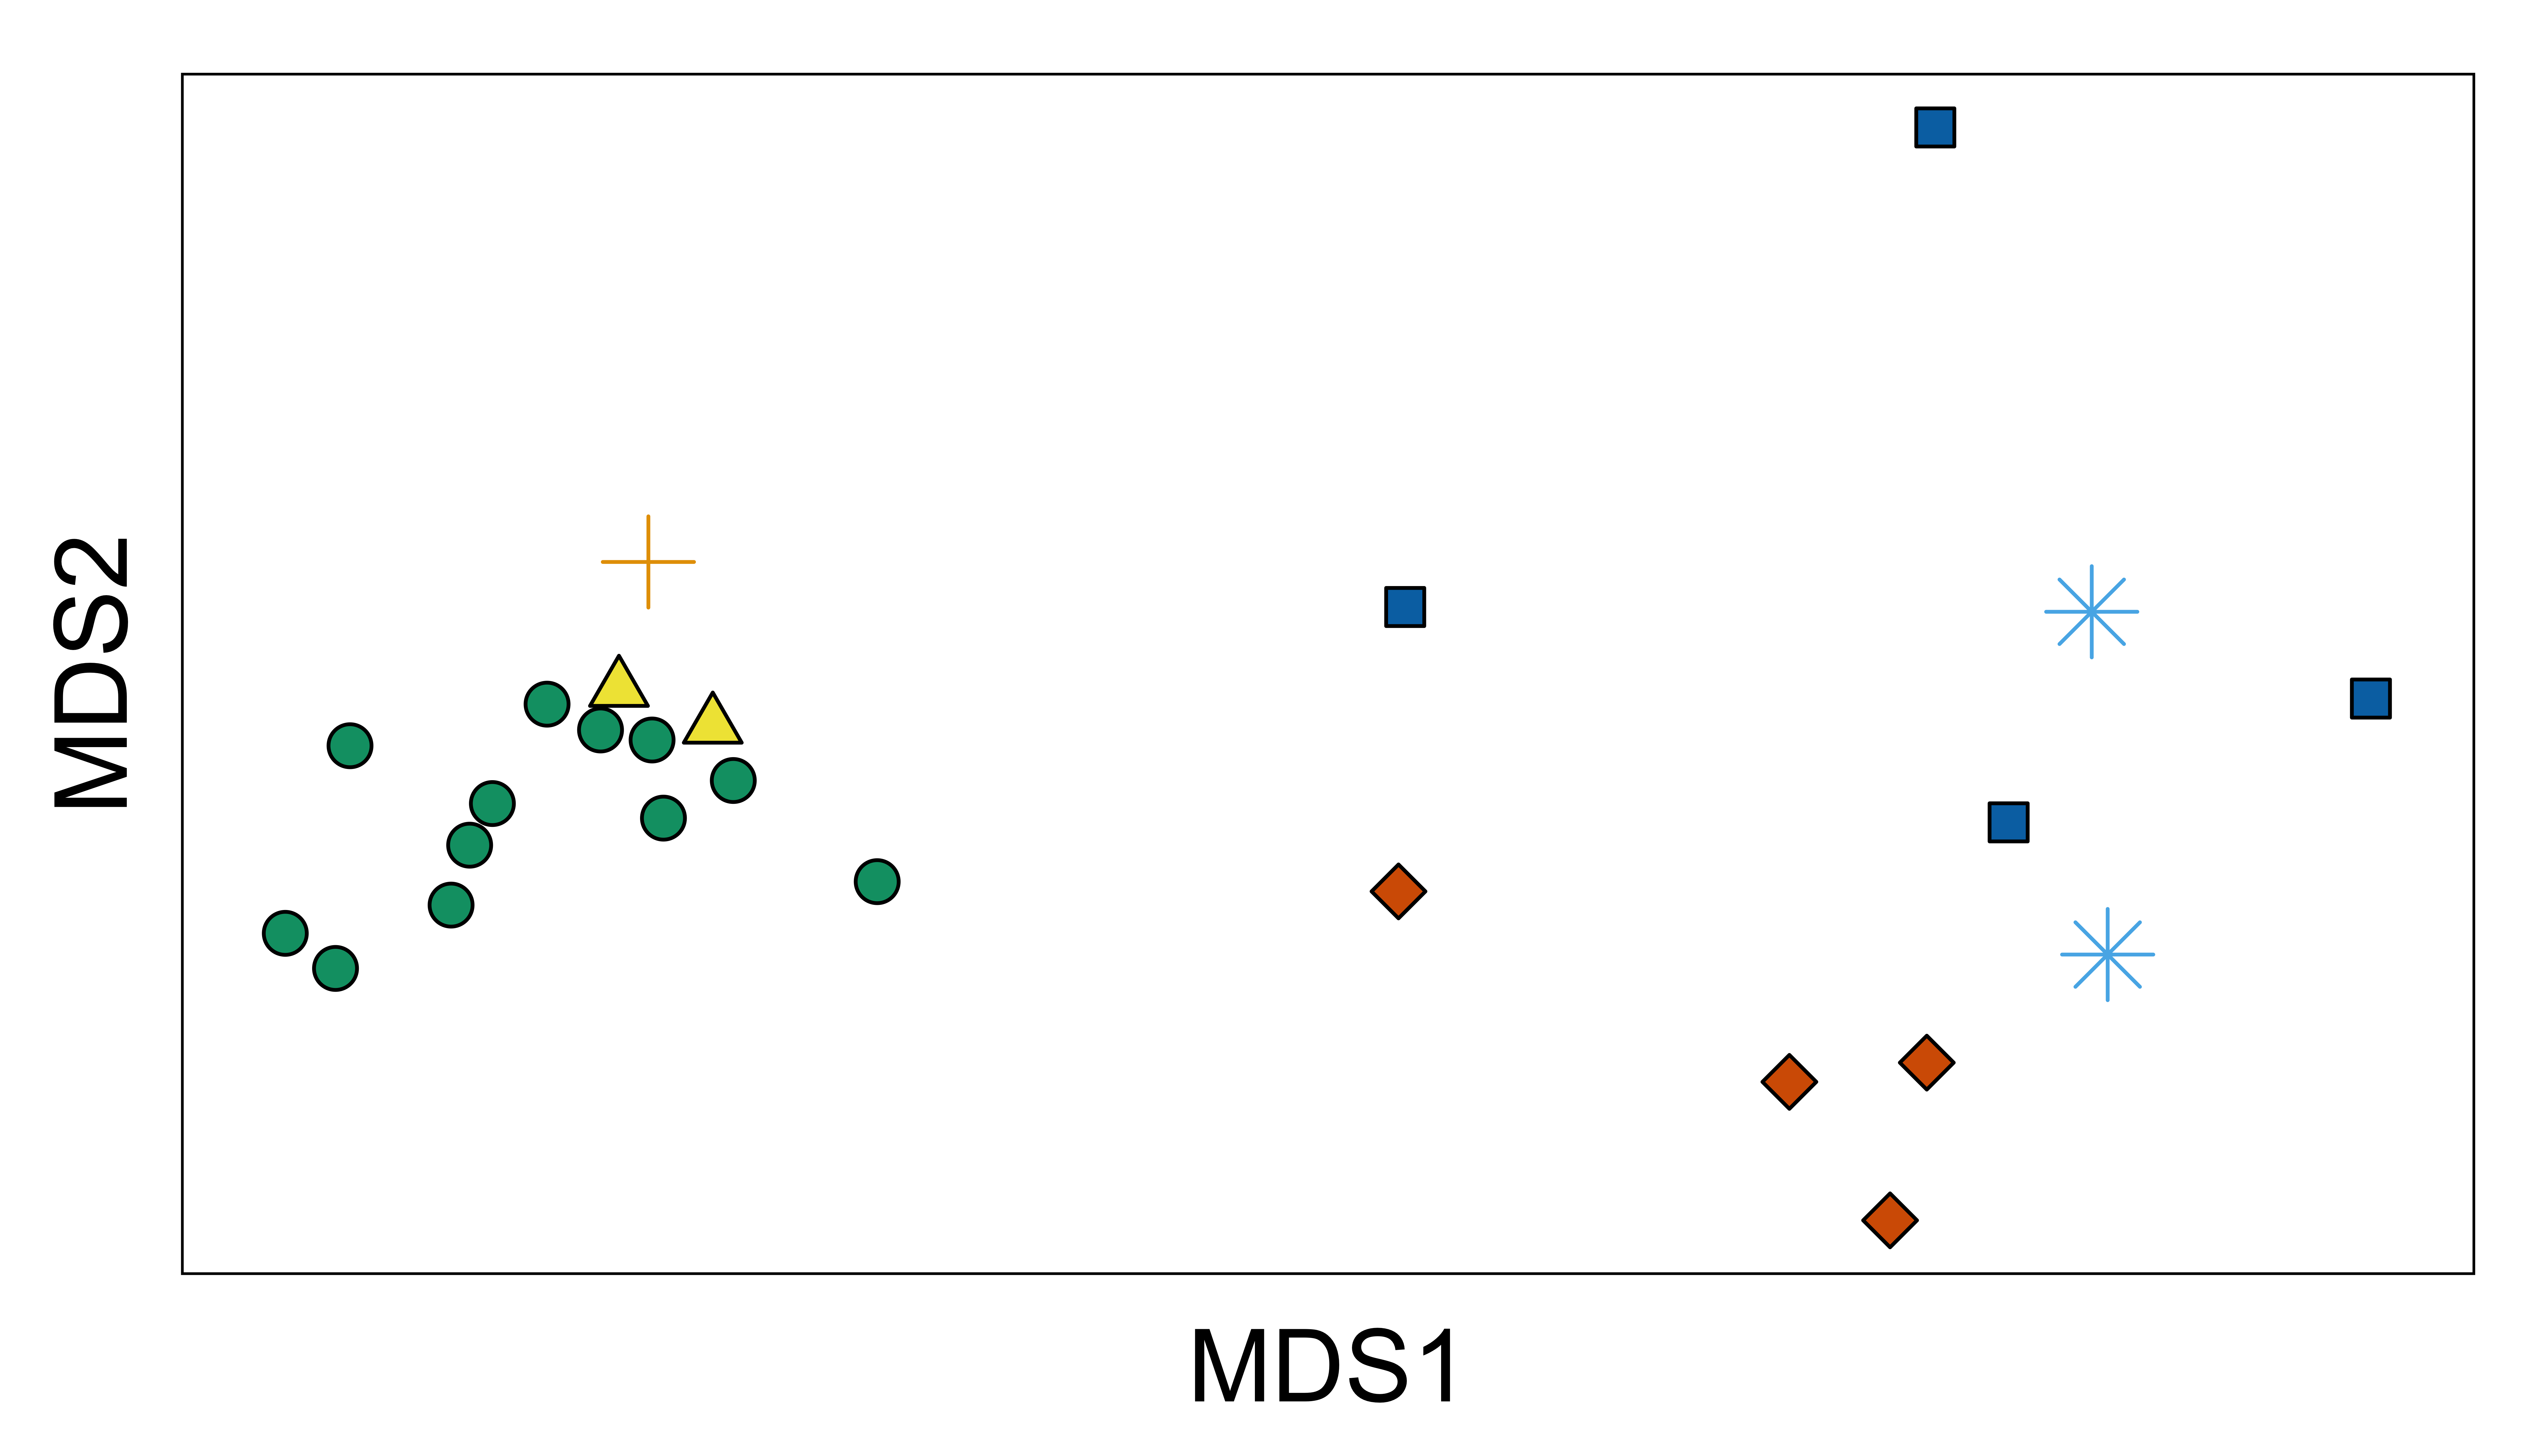
\includegraphics[width=\textwidth]{../advection/nMDStaxonomic.png}
  \caption[nMDS of advective distances between samples.]{nMDS ordination of the taxonomic distance matrix (2D stress = 0.08). Antarctic Intermediate Waters (AAIW), light blue stars; Subantarctic Mode Water (SAMW), orange crosses; Antarctic Bottom Water (AABW), dark blue squares; Antarctic Zone (AZ), green circles; Polar Frontal Zone (PFZ), yellow triangles; Circumpolar Deep Water (CDW), red diamonds.}
  \label{fig:nMDStaxonomic}
\end{figure}


\subsection{Environment and distance effects}
\ac{nMDS} ordination showed that the sampled water masses clustered well on the basis of environmental distance \figref{fig:nMDSenvironmental}.
This was supported by \ac{ANOSIM} (R = 0.84, p = 0.001). 
A partial Mantel test, comparing the taxonomic to environmental matrices with the spatial matrix held constant, found a correlation of r = 0.48 (p = 0.001), indicating a strong environment effect.

\begin{figure}[!ht]
  \centering
  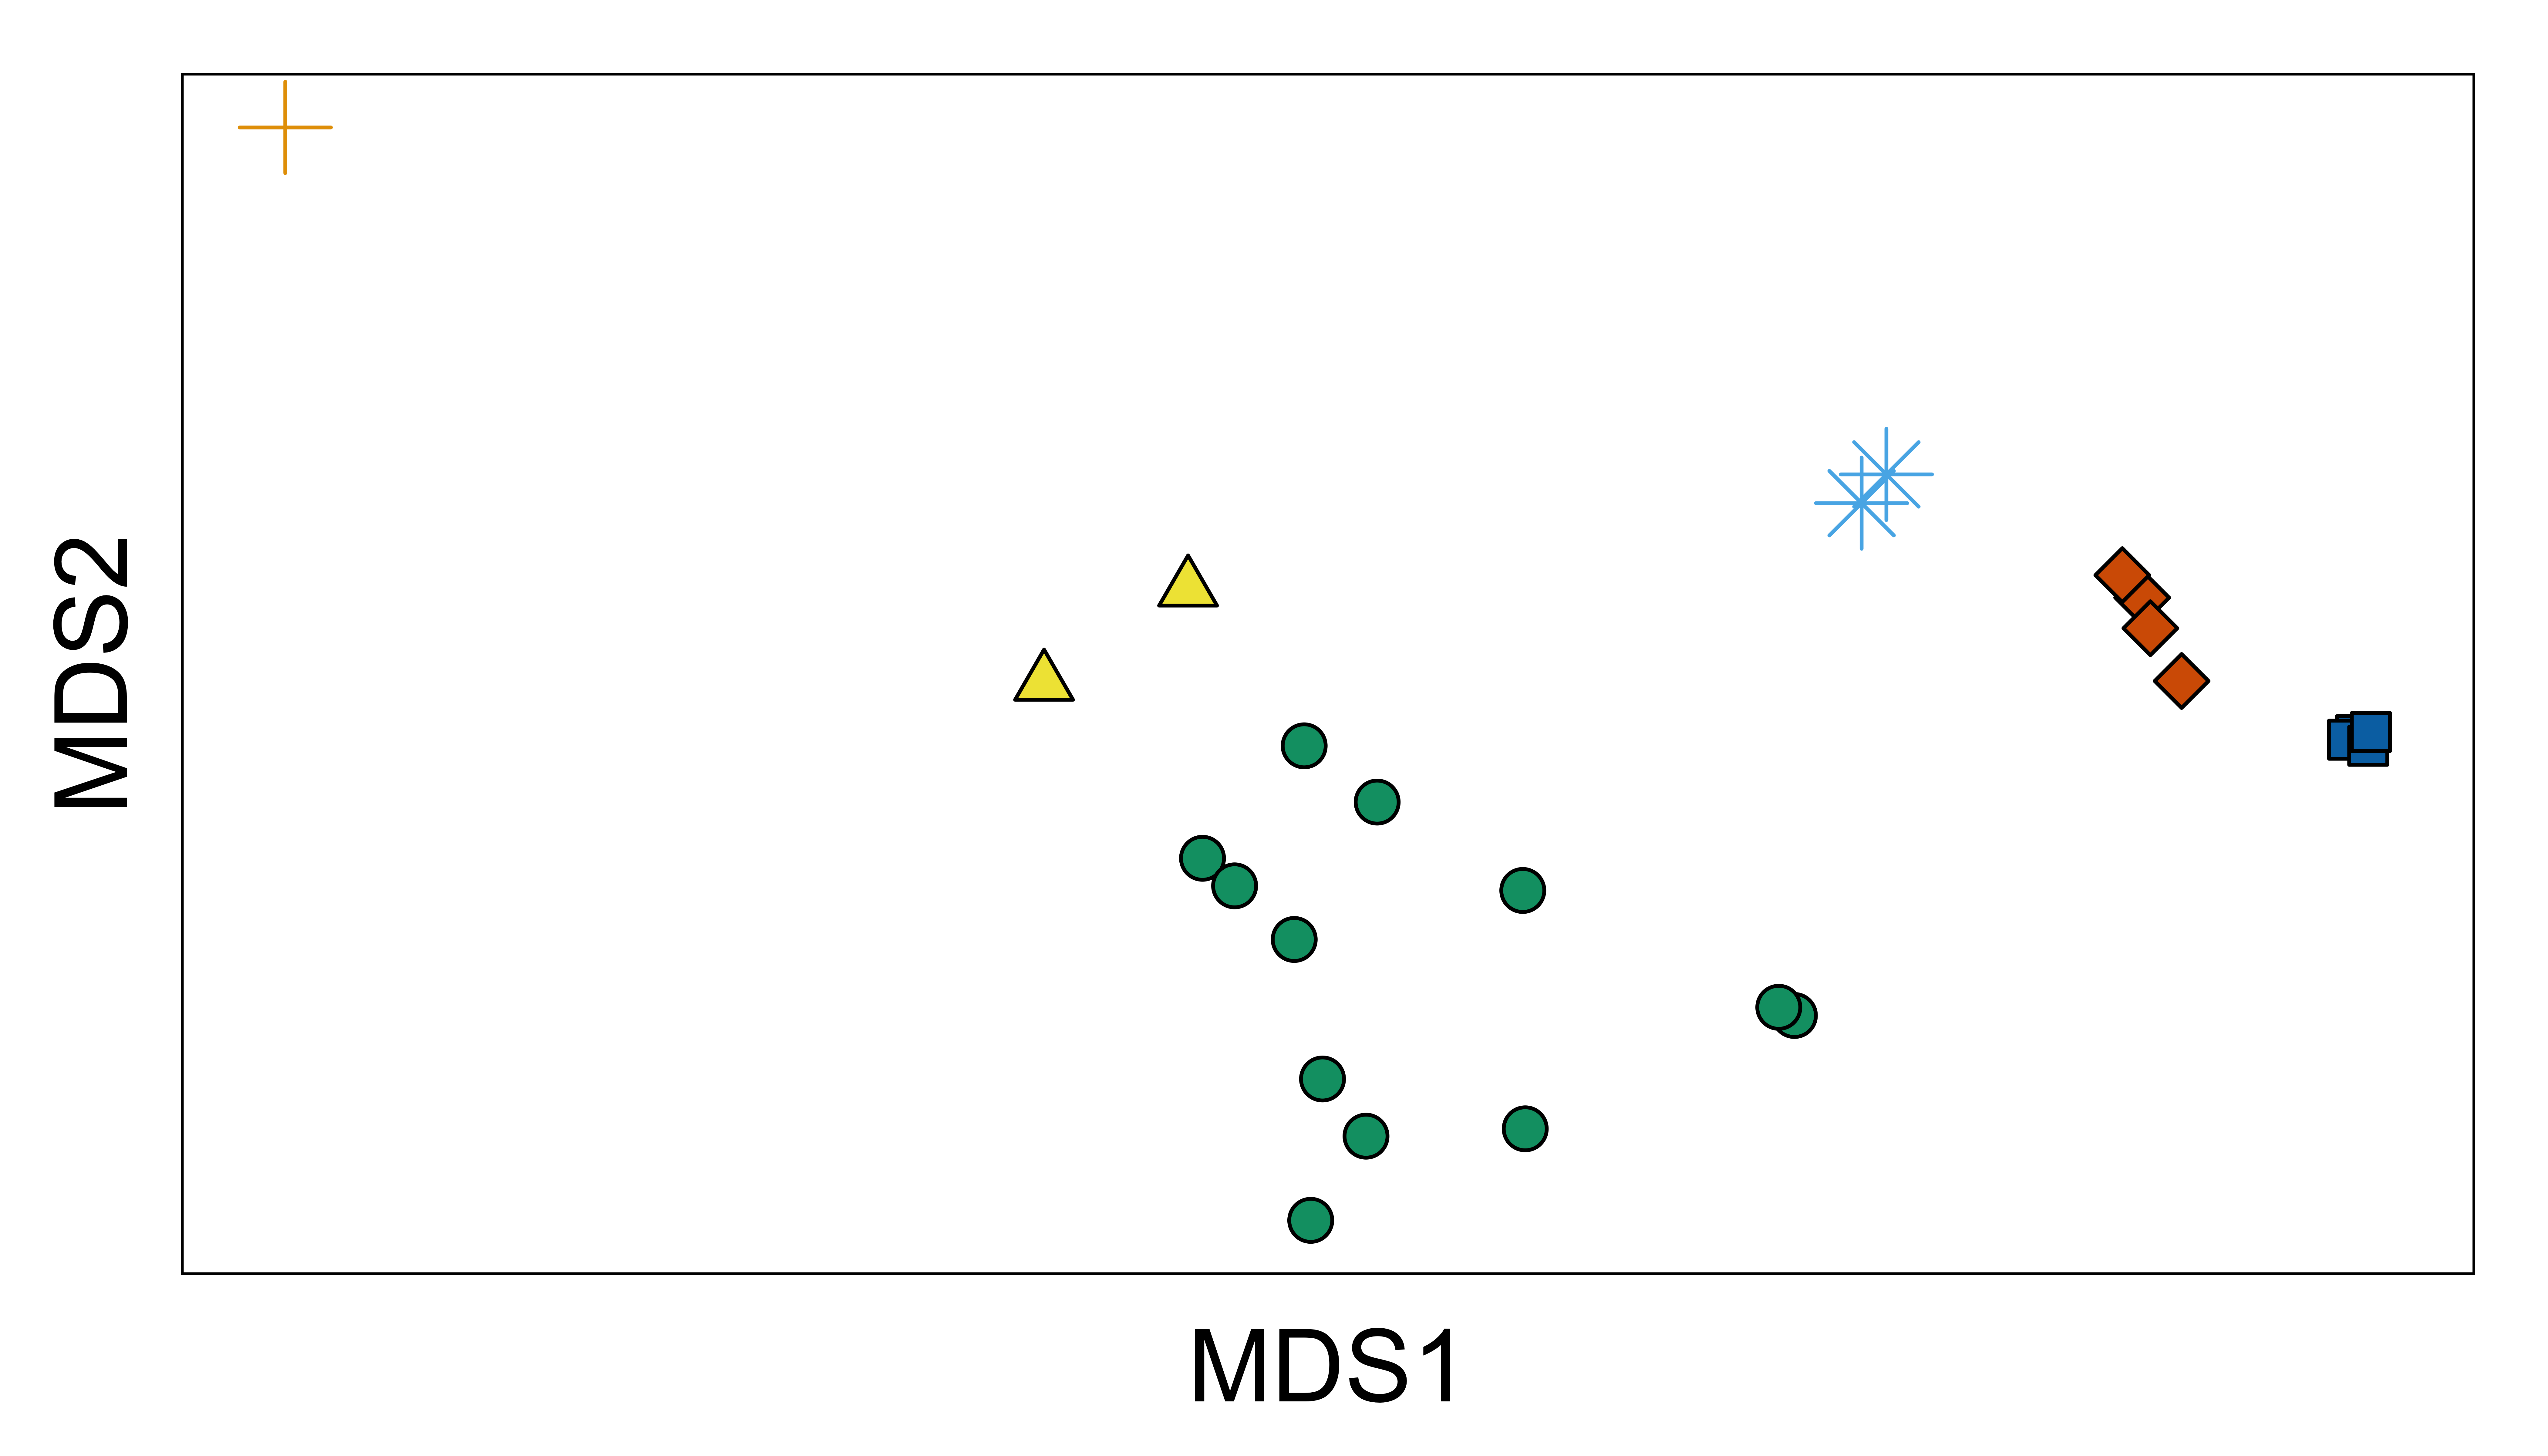
\includegraphics[width=\textwidth]{../advection/nMDSenvironmental.png}
  \caption[nMDS of advective distances between samples.]{nMDS ordination of the environmental distance matrix (2D stress = 0.02). Antarctic Intermediate Waters (AAIW), light blue stars; Subantarctic Mode Water (SAMW), orange crosses; Antarctic Bottom Water (AABW), dark blue squares; Antarctic Zone (AZ), green circles; Polar Frontal Zone (PFZ), yellow triangles; Circumpolar Deep Water (CDW), red diamonds.}
  \label{fig:nMDSenvironmental}
\end{figure}


\ac{distLM} analysis of the individual physicochemical variables found that considered separately, each of phosphate, silicate, nitrate, oxygen, salinity and pressure explained 17--35\% of the taxonomic variance between samples (p = 0.001).
Temperature had no significant effect on taxonomic composition when considered separately (p \textgreater{} 0.05).
When all combinations of variables were considered (BEST modelling), the best model consisted of all variables with the exception of phosphate (adjusted R\textsuperscript{2} = 0.44), with the full set of variables only marginally worse (adjusted R\textsuperscript{2} = 0.43).
The rejection of phosphate may reflect a redundancy in the measurement of both phosphate and nitrate; these are often held to be constant throughout the ocean at the Redfield ratio of N:P \textapprox{}16:1 \cite{Anderson:1994vb}.
However, deviation from this ratio has been observed in the \ac{SO} and related to iron concentration (which was not measured in this study) and to phytoplankton abundance \cite{Weber:2010fi}.
For these reasons, and because of the marginal effect of discarding phosphate from the variable selection, it was retained when generating the environmental distance matrix.

The \ac{dbRDA} plot showed the six variables retained by the \ac{distLM} model (i.e.\ all except phosphate) structured the samples first along an axis separating surface and deep samples (dbRDA1), strongly related to dissolved oxygen (r = 0.79) \figref{fig:dbRDA}.
The second axis was best correlated with temperature (r = \textminus{}0.75).
All six retained variables had a moderate correlation with at least one of the first two axes \tabref{tab:dbRDAcorrs}.
As with the \ac{nMDS} ordinations \figref{fig:nMDStaxonomic,fig:nMDSenvironmental,fig:nMDSadvection}, the water masses were generally well separated by the first two \ac{dbRDA} axes.
Samples from the \ac{AABW} and \ac{AAIW}, which were not separated by the first two axes, were clearly separated along the third \tabref{tab:dbRDAcorrs}, which was best correlated with pressure (r = \textminus{}0.79).
This suggests that these two masses had similar physicochemical properties, and were mainly distinguished by depth, consistent with their common origin in sinking Antarctic Surface Waters \cite{Foldvik:1988gp}.

\begin{figure}[!ht]
  \centering
  \includegraphics[width=\textwidth]{../advection/dbRDA.png}
  \caption[dbRDA ordination of relationship between environment and community.]{dbRDA ordination of the distLM model describing the relationship between the BEST-selected set of predictor physicochemical variables (pressure, oxygen, temperature, salinity, silicate, and nitrate) and the taxonomic dissimilarity between samples. Vectors represent the effect of each predictor variable on the two visualised axes. Vector length corresponds to the relative size of the effect, while direction represents the correlations to the two displayed axes. The first axis (dbRDA1) captures 64\% of fitted and 37\% of total variation between the samples' taxonomic profiles; the second (dbRDA2) captures 14\% of fitted and 8\% of total variation. Antarctic Intermediate Waters (AAIW), light blue stars; Subantarctic Mode Water (SAMW), orange crosses; Antarctic Bottom Water (AABW), dark blue squares; Antarctic Zone (AZ), green circles; Polar Frontal Zone (PFZ), yellow triangles; Circumpolar Deep Water (CDW), red diamonds.}
  \label{fig:dbRDA}
\end{figure}

\begin{table}[!ht]
\centering
\sffamily
\caption[Correlations between dbRDA axes and physicochemical variables]{Correlations between dbRDA coordinate axes and physicochemical variables (multiple partial correlations).}
\label{tab:dbRDAcorrs}
\begin{tabular}{lllllll}
\toprule
\textbf{Variable} & \textbf{dbRDA1} & \textbf{dbRDA2} & \textbf{dbRDA3} & \textbf{dbRDA4} & \textbf{dbRDA5} & \textbf{dbRDA6}\\
\midrule
Pressure & \textminus{}0.316 & \textminus{}0.485 & \textminus{}0.787 & \textminus{}0.148 & \textminus{}0.144 & \textminus{}0.048\\
Oxygen & 0.792 & \textminus{}0.171 & \textminus{}0.125 & 0.069 & \textminus{}0.567 & 0.050\\
Temperature & \textminus{}0.025 & \textminus{}0.750 & 0.366 & 0.236 & 0.180 & 0.463\\
Nitrate & \textminus{}0.311 & 0.007 & 0.325 & \textminus{}0.636 & \textminus{}0.561 & 0.281\\
Silicate & \textminus{}0.303 & 0.341 & \textminus{}0.166 & 0.615 & \textminus{}0.371 & 0.498\\
Salinity & \textminus{}0.290 & \textminus{}0.239 & 0.311 & 0.368 & \textminus{}0.417 & \textminus{}0.673\\
\bottomrule
\end{tabular}
\end{table}


A distance effect was detected by comparing the taxonomic and spatial matrices with the environmental matrix held constant (partial Mantel; r = 0.38, p = 0.003).
This indicated that a process other than contemporary environmental selection was appreciably affecting variation in microbial community composition.

\subsection{Testing the advection effect}

244,000 encounters were recorded between particles and sample sites during the 100 year advection simulation.
Encounter times spanned the full range of the simulation (5 days--100 years), with a median of 30 days and mean of 3018 days \figref{fig:encounterhistograms}.
47 pairs of samples did not yield mutual encounters (i.e.\ at least one particle from one sample encountering the other).
Of these, every pair included at least one AABW sample.

\begin{figure}
  \centering
  \includegraphics[width=\textwidth]{../advection/encounterhistogram1.png}
  \caption[Encounter times for all samples in advection model.]{Encounter times for all samples in advection model.}
  \phantomcaption
\end{figure}
  
\begin{figure}
  \ContinuedFloat
  \centering
  \includegraphics[width=\textwidth]{../advection/encounterhistogram2.png}
  \caption[]{(cont.) Encounter times for all samples in advection model.}
  \label{fig:encounterhistograms}
\end{figure}


\ac{nMDS} ordination showed that the sampled water masses could be broadly distinguished on the basis of their mutual advection distances \figref{fig:nMDSadvection}.
This was supported by \ac{ANOSIM} (R = 0.41, p = 0.002).

\begin{figure}[!ht]
  \centering
  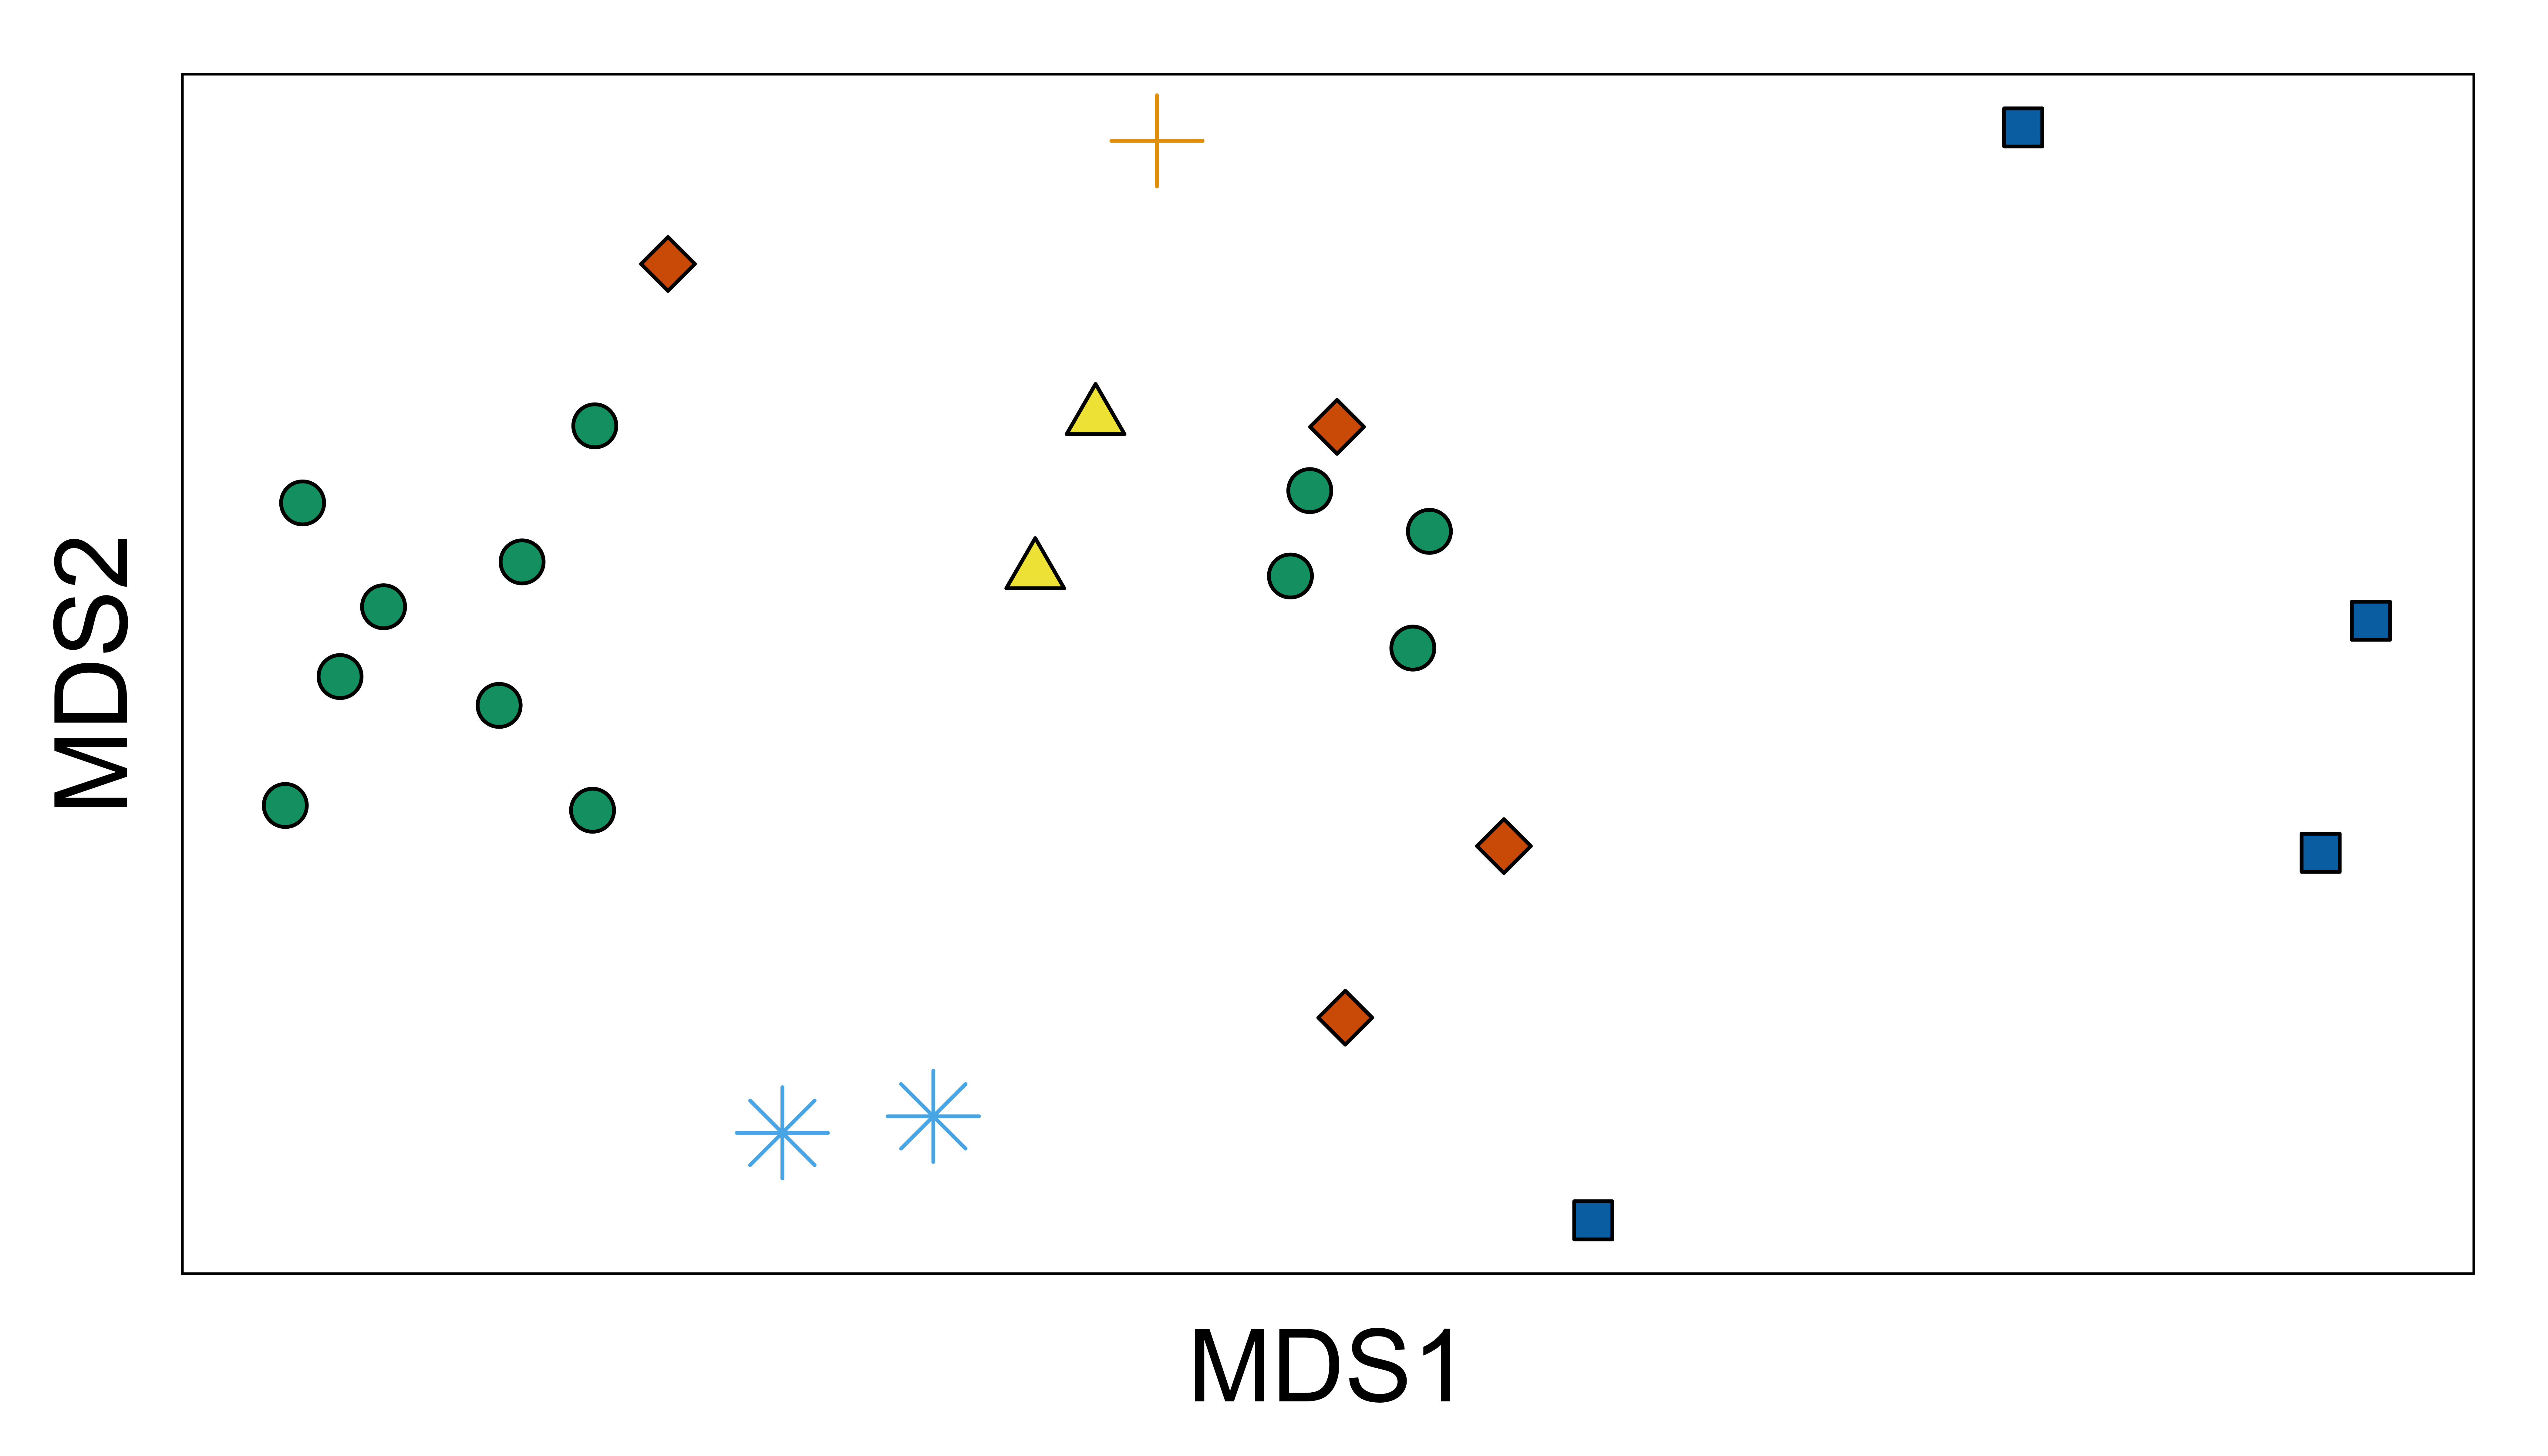
\includegraphics[width=\textwidth]{../advection/nMDSadvection.png}
  \caption[nMDS of advective distances between samples.]{nMDS ordination of the advection distance matrix (2D stress = 0.19). Antarctic Intermediate Waters (AAIW), light blue stars; Subantarctic Mode Water (SAMW), orange crosses; Antarctic Bottom Water (AABW), dark blue squares; Antarctic Zone (AZ), green circles; Polar Frontal Zone (PFZ), yellow triangles; Circumpolar Deep Water (CDW), red diamonds.}
  \label{fig:nMDSadvection}
\end{figure}


A partial Mantel test, comparing the taxonomic and advection matrices with the spatial and environmental matrices held constant, showed that advection has a moderate (r = 0.28) and significant (p = 0.010) correlation with taxonomic composition independent of spatial and environmental factors.
To ensure this result was not unduly influenced by the samples on which the 100 year ceiling was imposed (\ac{AABW}) and those for which particle releases were not simulated (samples 11, 13, 17 and 22), the test was repeated with these samples removed.
The correlation was stronger and remained significant despite the smaller sample size (r = 0.36, p = 0.025).
To ensure the result was robust to the choice of advection distance metric, correlations were recalculated for both the full set of samples and the subset (excluding \ac{AABW} and samples 11, 13, 17 and 22) with pairwise advection distance defined as the mean time for all particle encounters between samples.
The observed correlation was higher using this metric for both the full set (r = 0.40, p = 0.0090) and subset (r = 0.52, p = 0.0070).
\softwarename{SourceTracker} analysis confirmed that the effect was moderately directional, with the proportion of \acp{OTU} contributed from a given ``source'' sample to a ``sink'' sample correlated with the proportion of particle encounters it generates (Spearman's \textrho{} = 0.15, p = 0.0015). 

To explore the role of taxonomic resolution in the detection of an advection effect, partial Mantel tests were repeated as above with \acp{OTU} aggregated to each of the seven standard taxonomic ranks.
Aggregation to genus resulted in a higher correlation (r = 0.29, p = 0.02) than to species, but with this exception a pattern of decreasing correlation with coarser rank was observed \figref{fig:taxonomicresolution}.

\begin{figure}[!ht]
  \centering
  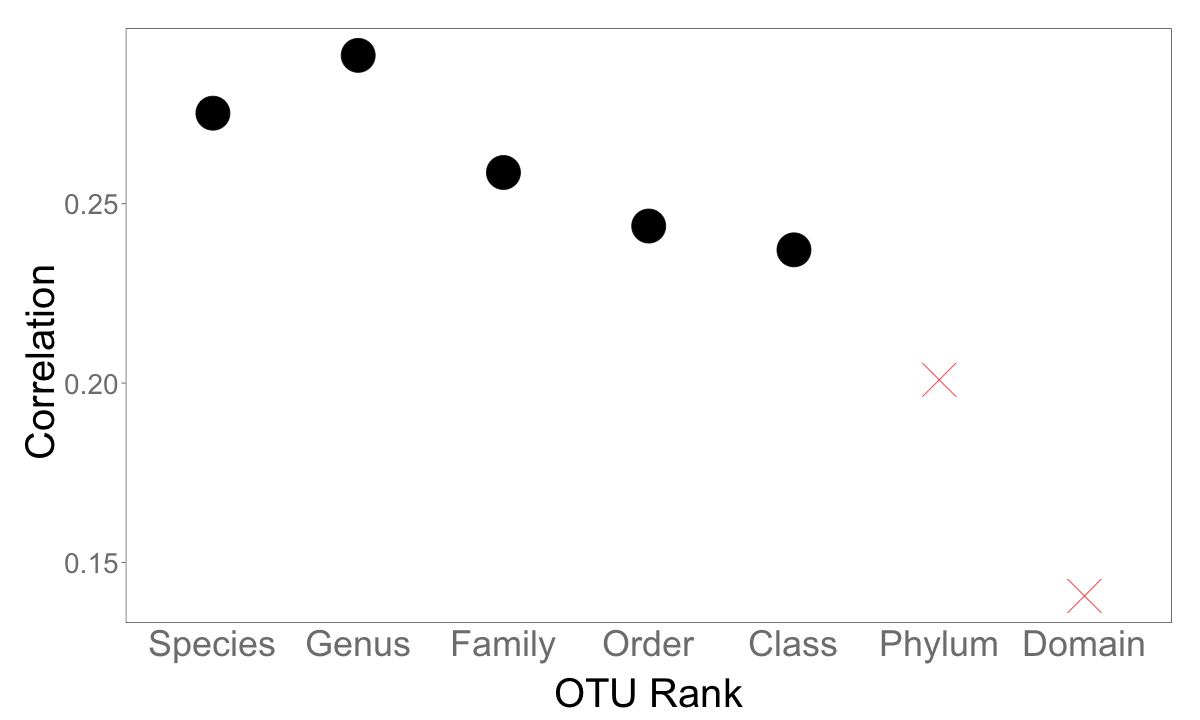
\includegraphics[width=\textwidth]{../advection/taxonomicresolution.png}
  \caption[Advection effect at different taxonomic resolutions]{Effect of taxonomic resolution on partial Mantel correlation between advection and taxonomic distances, with environmental and spatial distances held constant.
  Significant correlations (right-tailed p-value after 999 random permutations \textgreater{} 0.05), black circles; not significant correlations (\textlessthanorequal{} 0.05), red crosses.}
  \label{fig:taxonomicresolution}
\end{figure}


\subsection{Testing advection effect mechanisms}

Two explanations can be proposed for the relationship between advection and community composition.
The first is that advection increases microbial dispersal by increasing the probability that \acp{OTU} from one site will encounter and colonise another (the ``dispersal mechanism'').
This assumes microbial dispersal is less than perfect; i.e.\ that ``everything is not everywhere''.
The second is that advection transports a large numbers of cells at a rate measurably outpacing environmental selection, regardless of whether or not those cells are able to successfully colonise (i.e.\ grow and reproduce in) downstream sites: that ``the environment selects, but not fast enough'' (the ``bulk transport mechanism'').
Considering the long advection times between sites in this study, the relatively rapid growth of marine microorganisms, and the ability of small numbers of cells to rapidly reduce \textbeta{}-diversity between isolated marine sites \cite{Declerck:2013cz}, the dispersal mechanism seems the more plausible.

Two tests were performed to distinguish between these hypotheses.
Firstly, the advection distance matrix was reconstructed using the absolute pairwise number of particle encounters as the distance metric between samples (distance metric for given sample pair = maximum number of encounters across all sample pairs \textminus{} encounters for given pair + 1).
There was no significant correlation between this matrix and the taxonomic distance matrix when the environmental and spatial matrices were held constant (p \textgreater{} 0.05).
This suggests that advection time, not the absolute number of transported cells, is the relevant factor, supporting the dispersal mechanism.

Secondly, it was reasoned that under the dispersal mechanism, advection would have a large effect on the presence and diversity of taxa and a smaller effect on their abundances; while if the bulk transport hypothesis held, the effect would largely be on the relative abundances.
To test this, the taxonomic profiles were transformed to a presence/absence measure (\ac{OTU} present = 1, absent = 0), and a matrix of S\o{}rensen dissimilarities generated.
The advection effect was stronger (r = 0.33, p = 0.004) than when abundances were considered, again supporting the dispersal hypothesis. 

\subsection{Differential effect of advection on OTU subsets}

Over five restarts of the modified \softwarename{bvstep} algorithm, three (2, 4 and 5) produced the sample subset of four \acp{OTU} with correlation of 0.54 to the advection resemblance matrix (partial Mantel, p < 0.05) \figref{tab:bvstep}.
Restart 1 identified a different subset of 18 \acp{OTU}, also with a correlation of 0.54, while restart 3 identified a subset of 19 \acp{OTU} with a correlation of 0.44.
There was little overlap between the subsets: \speciesfull{Stenotrophomonas maltophilia} (0.8 \micron{} fraction) appeared in all subsets, while the alphaproteobacterium ``MGP-80'' (0.1 \micron{} fraction) appeared in all but restart 3.

\begin{table}[!ht]
\sffamily
\caption[Results of \softwarename{bvstep}]{OTU subsets resulting from five restarts of the modified \softwarename{bvstep} algorithm. OTUs common to more than one subset are indicated in {\color{red} red (all restarts)} or {\color{blue} blue (all restarts but 3)}.}
\label{tab:bvstep}
\begin{center}
\begin{tabular}{lll}
\toprule
& \textbf{OTU} & \textbf{Fraction (\micron)}\\
\midrule
Restart 1 & \speciesfull{Micrococcus luteus} NCTC 2665 & 3.0\\
&{\color{red} \speciesfull{Stenotrophomonas maltophilia}} & {\color{red}0.8}\\
&{\color{blue} Rhodobacteraceae bacterium MGP-80} & {\color{blue}0.1}\\
& \speciesfull{Cobetia marina} & 0.8\\
& Uncultured bacterium UCT N117 & 3.0\\
& Uncultured Marine Group II euryarchaeote DH148-W1 & 3.0\\
& Uncultured Bacteroidetes sp.\ & 0.8\\
& Uncultured \genus{Leeuwenhoekiella} sp.\ & 3.0\\
& \genus{Pseudoalteromonas} sp.\ NJSN44 & 0.1\\
& Rhodobacteraceae bacterium MGP-80 & 0.8\\
& \speciesfull{Zunongwangia profunda} SM-A87 & 3.0\\
& Uncultured \genus{Granulicatella} sp.\ & 3.0\\
& Uncultured \genus{Marinicella} sp.\ & 3.0\\
& Uncultured \genus{Oleiphilus} sp.\ & 3.0\\
& Uncultured \genus{Zunongwangia} sp.\ & 0.8\\
& \genus{Granulicatella} sp.\ & 3.0\\
& Uncultured \genus{Crocinitomix} sp.\ & 0.8\\
& \genus{Serratia} sp.\ 8H1D & 0.1\\
\midrule
Restarts 2, 4 and 5 & Uncultured \genus{Rhodococcus} sp.\ & 0.1\\
& \speciesfull{Leeuwenhoekiella blandensis} MED217 & 3.0\\
& {\color{blue} Rhodobacteraceae bacterium MGP-80} & {\color{blue}0.1}\\
& {\color{red} \speciesfull{Stenotrophomonas maltophilia}} & {\color{red}0.8}\\
\midrule
Restart 3 & Uncultured \genus{Singulisphaera} sp.\ & 3.0\\
& \genus{Mariniflexile} sp.\ HWR-17 & 3.0\\
& Uncultured \genus{Pelomonas} sp.\ & 0.8\\
& Uncultured \genus{Marinobacter} sp.\ & 3.0\\
& Uncultured bacterium KM3-205-D9 & 0.8\\
& \genus{Sphingobium} sp.\ SKA58 & 0.8\\
& \genus{Marinobacter} sp.\ 114Z-23 & 0.8\\
& Uncultured Bacteroidetes bacterium NS2b & 0.8\\
& Uncultured \genus{Marinicella} sp.\ & 3.0\\
& {\color{red} \genus{Stenotrophomonas maltophilia}} & {\color{red}0.8}\\
& Uncultured \genus{Hirschia} sp.\ & 3.0\\
& BD2-11 terrestrial group uncultured bacterium AD254-A9 & 0.8\\
& \speciesfull{Kocuria rhizophila} DC2201 & 0.8\\
& Uncultured \genus{Vibrio} sp. & 0.8\\
& Uncultured bacterium & 3.0\\
& Uncultured marine crenarchaeote AD1000-23-H12 & 0.1\\
& Uncultured marine group III euryarchaeote & 3.0\\
& \genus{Halomonas} sp. HK31 & 0.8\\
& Uncultured Acidobacterium sp.\ DA023 & 0.1\\
\bottomrule
\end{tabular}
\end{center}
\end{table}


\section{Discussion}

This study found good support for the hypothesis that advection shapes microbial assemblages independent of an environment or distance effect.
Communities that are more closely connected by advection are more similar, and this effect exists even when environment and distance effects are controlled for.
The results also indicate that advection primarily shapes microbial community structure by increasing opportunities for colonisation, rather than transporting large numbers of cells to downstream sites. 

The major alternative hypothesis for the observed correlation is that there exists an unmeasured environmental variable (e.g.\ iron concentration, pH) which correlates well with both advection and community composition.
As in all studies of historical influences on microbial biogeography, it is impossible to eliminate all potential confounding variables.
However, a rigorous confirmation of the advection effect will require future work to measure physicochemical parameters as comprehensively as possible.

The amount of variance in taxonomic composition explained by the advection effect can be estimated as the square of the correlation coefficient (r\textsuperscript{2}).
This value, 7\%, is likely to be a conservative estimate, as this study only captured advective pathways from one sample to another; it is possible that some samples with a large mutual advective distance shared a common advective source outside the study area.
A recent review of studies partitioning variance in microbial community composition found that the mean reported variance explained by a distance effect was 10\%, and by an environment effect 27\% \cite{Hanson:2012cb}.
The estimated proportions of variance in this study, 14\% (p = 0.001) for distance and 23\% (p = 0.001) for environment, were close to these values.
While there are no comparative data for the advection effect in other systems, the value of at least 7\% for the \ac{SO} indicates that advection is important relative to both distance and environment effects. 

\subsection{Taxonomic resolution}

Taxonomic resolution (i.e.\ the level of genetic difference at which \acp{OTU} are discriminated) often determines whether or not a pattern is detected in studies of microbial distance effects, with finer resolutions generally leading to an increased likelihood of detecting a significant effect \cite{Hanson:2012cb}.
Surprisingly, aggregation to genus resulted in a higher correlation than to species \figref{fig:taxonomicresolution}.
This may be because of the selection of the V6--V8 hypervariable regions as the sequencing target.
Amplification of the V6 region alone has been shown to underestimate species richness, while targeting the V7--V8 region overestimates it \cite{Youssef:2009un}.
It is possible that due to this choice of target, the ``species''-level aggregation represents a much finer taxonomic resolution at which intra-species variability begins to overwhelm the advection effect.
With this exception, the pattern of a decreasing effect with coarser taxonomic resolution was confirmed, with no statistically significant effect for aggregation to phylum or domain.

\subsection{Differential influence of advection on OTU subsets}

The attempt to identify subsets of \acp{OTU} which were more amenable to advection produced inconclusive results.
While three almost unique subsets were identified \tabref{tab:bvstep}, all of which had a stronger correlation with advection distance than the complete set, there was no clear pattern in the \acp{OTU} selected.
For example, it was hypothesised that organisms capable of dormancy (e.g.\ spore formation) might be more amenable to advective transport as they would be more likely to survive over long distances and travel times.
However, there was no obvious overrepresentation of such taxa in the results.
Most selected \acp{OTU} were uncultured, and had very low estimated relative abundances, further complicating interpretation.

It is possible that the very large number of \acp{OTU} identified in this study means that any with a strong correlation to advection were outnumbered by those correlating through random chance.
These results illustrate the difficulty of translating patterns on the ecosystem or biogeographic level into descriptions of individual species.

\subsection{Future work}

To obtain a better understanding of the advection effect, it would be useful to determine whether particular taxonomic or physiological groups are more amenable to dispersal by advection; e.g.\ through the formation of dormant spores \cite{Sul:2013in, Bissett:2010wj}.
As it is possible that an unmeasured environmental variable (e.g.\ iron concentration, see Discussion) also correlates with both advection and community composition, future studies should address this.
Finally, further mesocosm experiments like those reported by \citet{Declerck:2013cz} will be useful to confirm the effect of small-scale exchange of cells between sites on colonisation and community structure.
